\section{Topological quantum order}

\subsection{Overview}

\subsubsection{Introduction}

In this chapter we will be giving a detailed analysis of topological quantum order, a particular type of topological quantum system. We recall below how this fits into the general framework of this book:

\begin{equation*}
\tikzfig{mathematical-outline-TQO}
\end{equation*}

Topological quantum systems are distinguished by the fact that their states don't depend on local properties - they depend only on global topological properties of the system. One way of getting this sort of topological invariance is through \textit{discreteness}. If a system is discrete, all of its parts are in a sense \textit{far away} from each other. Things which are far away cannot be continusly deformed from one to another - local changes can't change discrete objects. A real-number valued invariant could move all over the place and depend heavily on local properties of a system, but an integer-valued invariant is \textit{neccecarily} topological invariant.

We demonstrate this below in its most basic form. Suppose that $V$ is a Hilbert space and $H:V\to V$ is a Hermitian operator. This represents a quantum system and its Hamiltonian. Let $\ket{\psi}$ be an energy eigenstate with energy $E$. Suppose further that the $E$-eigensapce of $H$ is one dimensional, and that every other eigenvalue $E'$ on $H$ satisfies $|E'-E|\geq \Delta$ for some real number $\Delta>0$. This situation is demonstrated in the below graph:

\begin{equation*}
\tikzfig{TQO-spectrum-1}
\end{equation*}

This energy gap around $E$ adds a sort of discretness to the spectrum of $H$. Suppose that the system is in state $\ket{\psi}$ and we distort it a small amount. Typically, \textit{this will not affect the state}. The state $\ket{\psi}$ would need to jump all the way to some other state, but all other states have significantly different energies. In particular, if the perturbation applied to $\ket{\psi}$ has magnitutde significatly less than $\Delta$, then $\ket{\psi}$ cannot change. This connection between gaps in energy spectra and topological states is so essential that many physicists use the terms \textit{topological system} and \textit{gapped system} interchangably. 

So, in practice, how do we make sure that the perturbations being applied to $\ket{\psi}$ are always much smaller than $\Delta$? We make the system \textit{cold}. Roughly we say that a system has \textit{temperature} $T$ if the states of the Hamiltonian being occupied all have energy $<T$, and perturbations from the environment have magnitute $\approx T$. We renormalize our Hamiltonain so that the lowest energy eigenstate has energy $0$. We call the lowest energy eigenstates the \textit{ground states} of the system. We now assume that the ground state space is one dimensional, so there is a unique ground state. We assume that the next lowest energy eigenvalue is $\Delta>0$. This gives us a new picture:

\begin{equation*}
\tikzfig{TQO-spectrum-2}
\end{equation*}

So long as the temperature is much smaller than the energy gap ($T\ll \Delta$), then our system will remain in the ground state. We say that the system $(V,H)$ \textit{becomes topological at low temerature}. 

Of course, there's a big problem in our above discussion. \textit{Every} finite dimensional quantum system is gapped. The Hamiltonian has finitely many eigenvalues, so its spectrum is neccecarily discrete. What we should really be imagnining is an infinite family of systems, paramaterized by some real number $L>0$ called the \textit{linear system size}. Working in a two dimensional system, this will look like the below picture:

\begin{equation*}
\tikzfig{system-size}
\end{equation*}

Letting $\dim(V)$ denote the dimension of $V$, this gives us an assymptotic formula $\dim(V)\sim e^{(\text{const})\cdot L^2}$ where the constant in the exponent depends on the density of quantum degrees of freedom in the system. Let $\Delta_L$ be the lowest nonzero energy of the Hamiltonian in the size-$L$ system. Of course, we will always have a gap $\Delta_L>0$. What's important is that we require that $\Delta_L>\Delta$ for some uniform $\Delta>0$. In most quantum systems this will \textit{not} be there case - as the system size gets larger there will be states with smaller and smaller nonzero energies.

The issue with our discussion up to now is that it is \textit{no use} for making a topological quantum computing. There is only a single ground state, so there is no non-trivial topologically protected information. There's just a point. To make a quantum computer we will need to introduce \textit{degeneracy} into the ground states - make the lowest energy eigenspace higher dimensional. This degenerate ground space is where we will store our information.

If we do this naively, there's an immediate issue which appears. What if a perturbation of the system keeps the vectors in the ground space, but perturbs exactly which vector in the ground space is being stored. Wouldn't this corrupt the data? The trick is choose the ground space correctly so that this does not happen. The way this works is by choosing a ground space which has a basis consiting of vectors which are in a certain sense ``far apart". Because they are far apart, they cannot easily be distored from one to another.

More explicitley, let us choose standard basis $S$ for $V$, inducing an isomorphism $V= \CC[S]$. This basis should correspond to the physical degrees of freedom underlying the system. If $V$ is made up of an $L$ by $L$ grid of some repeating quantum sub-system, then choosing some arbitary basis $D$ for that subsystem a good choice for $S$ is $D^{L^2}$, coming from the isomorphism $\CC[S]\cong \CC[D]^{\otimes L^2}$ where $\otimes$ in the exponent denotes repeated tensor product. The canonical metric on $\CC$ induces a product metric on $V=\CC[S]$. It is with respect to this topology that we want our basis for the ground space to be far apart. That is, we require a basis $B$ for the ground space such that for every $b_1,b_2\in B$, $|b_1-b_2|$ is large. The exact scale of large depends on the topological system. At the very least it should tend to ininity with system size. In this case we will require an exponential scaling, $|b_1-b_2|>e^{(\text{const})L}$:

\begin{equation*}
\tikzfig{TQO-basis-distance}
\end{equation*}

[WORK: this stuff about distance is totally bogus. The real point is that if you differ at a large number of sites then it neccecarily takes a large number of local errors to make a difference! Probability gets exponentially suppressed. Global feature $\implies$ touches $>(\text{const})\cdot L$ sites.]

This allows us to state a full picture of how to store topological information in a gapped system. Suppose we have some gapped system as before with distinguished geometric basis $S$, Hilbert space $V=\CC[S]$, Hamiltonian $H$, temperature $T$, topological energy gap $\Delta$, and linear system size $L$. We suppose $T\ll \Delta$, $L\gg 0$. Suppose further that the information we wish to store is the ground state

$$\ket{\psi}=\sum_{x\in S}c_x \ket{x}.$$

As time goes, we image the coefficents $c_x$ continuously varying due to noise. This noise should have magnitute $\cong T$. We control our information by repeately measuring with repsect to $H$. This measurement continually projects the our information back into an eigenstate. This is a mathematical mechanism for \textit{cooling} - keeping the energy low. A few things could happen when $H$ is measured.

\begin{enumerate}
\item Typically, after measuring the state will be projected back into the ground state space. The stored information will change a small continuous amount. The magnitute of this change is on the order of $T/e^{(\text{const})L}$. This is because basis vectors in the ground space are on the scale of $e^{(\text{const})L}$ times further apart than the basis vectors of $\CC[S]$. Hence, the metric on the ground space is dialated by a factor of $e^{(\text{const})L}$, which has the effect of dampening the magnitute of the drift. Even though our stored information is always being corrupted by noise, the magnitute of this noise is tiny. Making the system size large, we can efficently make the drift arbitaraily small. For any polynomial-length algorithm, the total amount of drift is still suppressed to large enough degree that the errors are tolerable. This means that our information is \textit{topologically protected} in this case.

\item After measurement, the state could get projected onto an energy eigenstate which is \textit{not} a ground state. This corresponds to a spontanous jump in energy. The probability of such a jump is suppressed by the magnitute of the gap, giving a probability on the order of $T/\Delta$. Choosing $T\ll \Delta$, we can make this probability small. However, we cannot make it arbitrarily small, and errors of this type need to dealt with as they will surely appear in any sufficently long algorithm. The upside is that when these errors occur it is entirely detectable - the outcome of the measurement of $H$ is some observable energy, and it can be detected when that energy becomes nonzero. When it is detected that the energy is nonzero, then the experimenters can project the system back into the ground space by applying some external probe. The experiments can choose this projection carefully so that it sends the state to the nearest ground state, keeping the information drift on the order $T/e^{(\text{const})L}$. The details of how experimenters project non-ground states into ground states depends from topological system to topological system, and is often the heart of a proposal for topological quantum computing.
\end{enumerate}

All in all, we find that following the procedures outlined above we can store topological information with essentially no errors. This is topological quantum memory.

The question now is how to make a \textit{computer} of this. How do you act on the information stored this way in a gapped system? How do we go from one state to another in a topologically protected way? There are lots of different ways to do this, each of which have many equivalent descriptions. Here I will present a framework similar to the one introduced by Aasen-Wang-Hastings \cite{aasen2022adiabatic}. In this framework, we perform computations by slowly transformation which Hamiltonian $H$ we use to cool the system.

Suppose we have some state $\ket{\psi}$ we want to perform our computation on. We will choose some a family of Hamiltonians $H_t$, one for each time $t\in [0,1]$. We will require that $H_0=H_1=H$ is our original Hamiltonian. We will continuously transform which Hamiltonian we use to cool the system. That is, at every time step $t$, we measure the system with repsect to the Hamiltonian $H_t$. Assuming that the Hamiltonians vary slowly enough, our comments above apply. Namely, at time $t$ either the state will stay a ground state of $H_t$ with minimal drift or it will spontanously jump to an excited state. In the case that it jumps to an excited state, we can apply an external probe to project it back into a ground state. Letting $\ket{\psi(t)}$ denote the state at time $t$, we find that $\ket{\psi(1)}$ will be some new ground state of $H$, which is well-defined up to errors on the scale $T/e^{(\text{const})L}$.

The beautiful observation is that $\ket{\psi(1)}$ does not need to be equal to $\ket{\psi(0)}=\ket{\psi}$. If the path taken by the Hamiltonains is non-trivial it can have a non-trivial action on the ground states, and serve as a source of computation. This is topological quantum computation. This sort of continuous evolution of a Hamiltonian while keeping a state in the ground state is known as an \textit{adiabatic} evolution of the Hamiltonian. An important point to emphaize is that for the above procedure to work, the Hamiltonians $H_t$ must all have energy gaps, and these gaps must all be bounded below. Namely, $>\Delta$ for a fixed $\Delta$. This model of computation can be summarized as saying that computations are performed by adiabatically transforming the Hamiltonian along non-trivial paths in the configuration space of all possible gapped Hamiltonians.

This already allows us to make interesting comments about the nature of topological quantum computing. To make a powerful quantum computer, there needs to be a lot of different loops that the Hamiltonian can go around, corresponding to a lot of possible different gates that can be applied. This means that the path-connected component of the original Hamiltonian in the configuration space of all possible gapped Hamiltonians has to have lots of non-trivial loops - its fundamental group needs to be large. Choosing gapped Hamiltonains whose path connected component in the space of gapped Hamiltonians has interesting topology is the art of topological quantum computing. It is here that we can get the definition of what a topological order is. It is a path connected component in the configuration space of gapped Hamiltonians. Or, equivalently, an equivalence class of gapped Hamiltonian up to continuous deformation.

Note that the exact definition of gapped Hamiltonian is subtle, because really we are talking about infinite families of Hamiltonians paramaterized by system size, and so our above definiitons of topological order are only approximate. The point is that topological order captures the inherent algebraic structure and nontrivial topology with a gapped Hamiltonian, while forgetting the details of how that Hamiltonian is defined.

[WORK: How should I define topological order, as opposed to simply ``gapped Hamiltoninan"? What am I missing? Is this something I even want to define it? Add a subsection?]

[WORK: The papers \cite{cui2020kitaev, bravyi2010topological,bravyi2011short} all agree on two axioms of TQO, TQO-1 and TQO-2. The exact implementation of these axioms are different, but their philosophy is here. Bring them in.

TQO-1 = ground states are error correcting code (topological protection)

TQO-2 = local ground state coincides with global one (allows for quasiparticle picture)

]

\subsection{Discrete gauge theory}

\subsubsection{Ordered media on a lattice}

Above we defined topological order. The best way to demonstrate the general prinmciples of topological order is to give a good family of examples. The examples we will give in this section come from \textit{discrete gauge theory}. At its heart, discrete gauge theory is a quantum version of the notion of ordered media we defined in Chapter [ref] section [ref]. While mathematically unnececary, the next two subsections give physical motivation for why the formulas for discrete gauge theory have to be like they are, and why their analysis behaves like it does. Those who feel comfortable working with unmotivated formulas should skip to subsection [ref].

We will go from ordered media to discrete gauge theory in two steps:

\begin{enumerate}[Step 1:]
\item Put ordered media on a lattice;
\item Make it quantum.
\end{enumerate}

This first subsection is focused on Step 1. We will do Step 2 in the next subsection.

The first natural question to ask is \textit{what is a lattice}. For our purpose a lattice is something like the picture below:

\begin{figure}[h]
\begin{center}
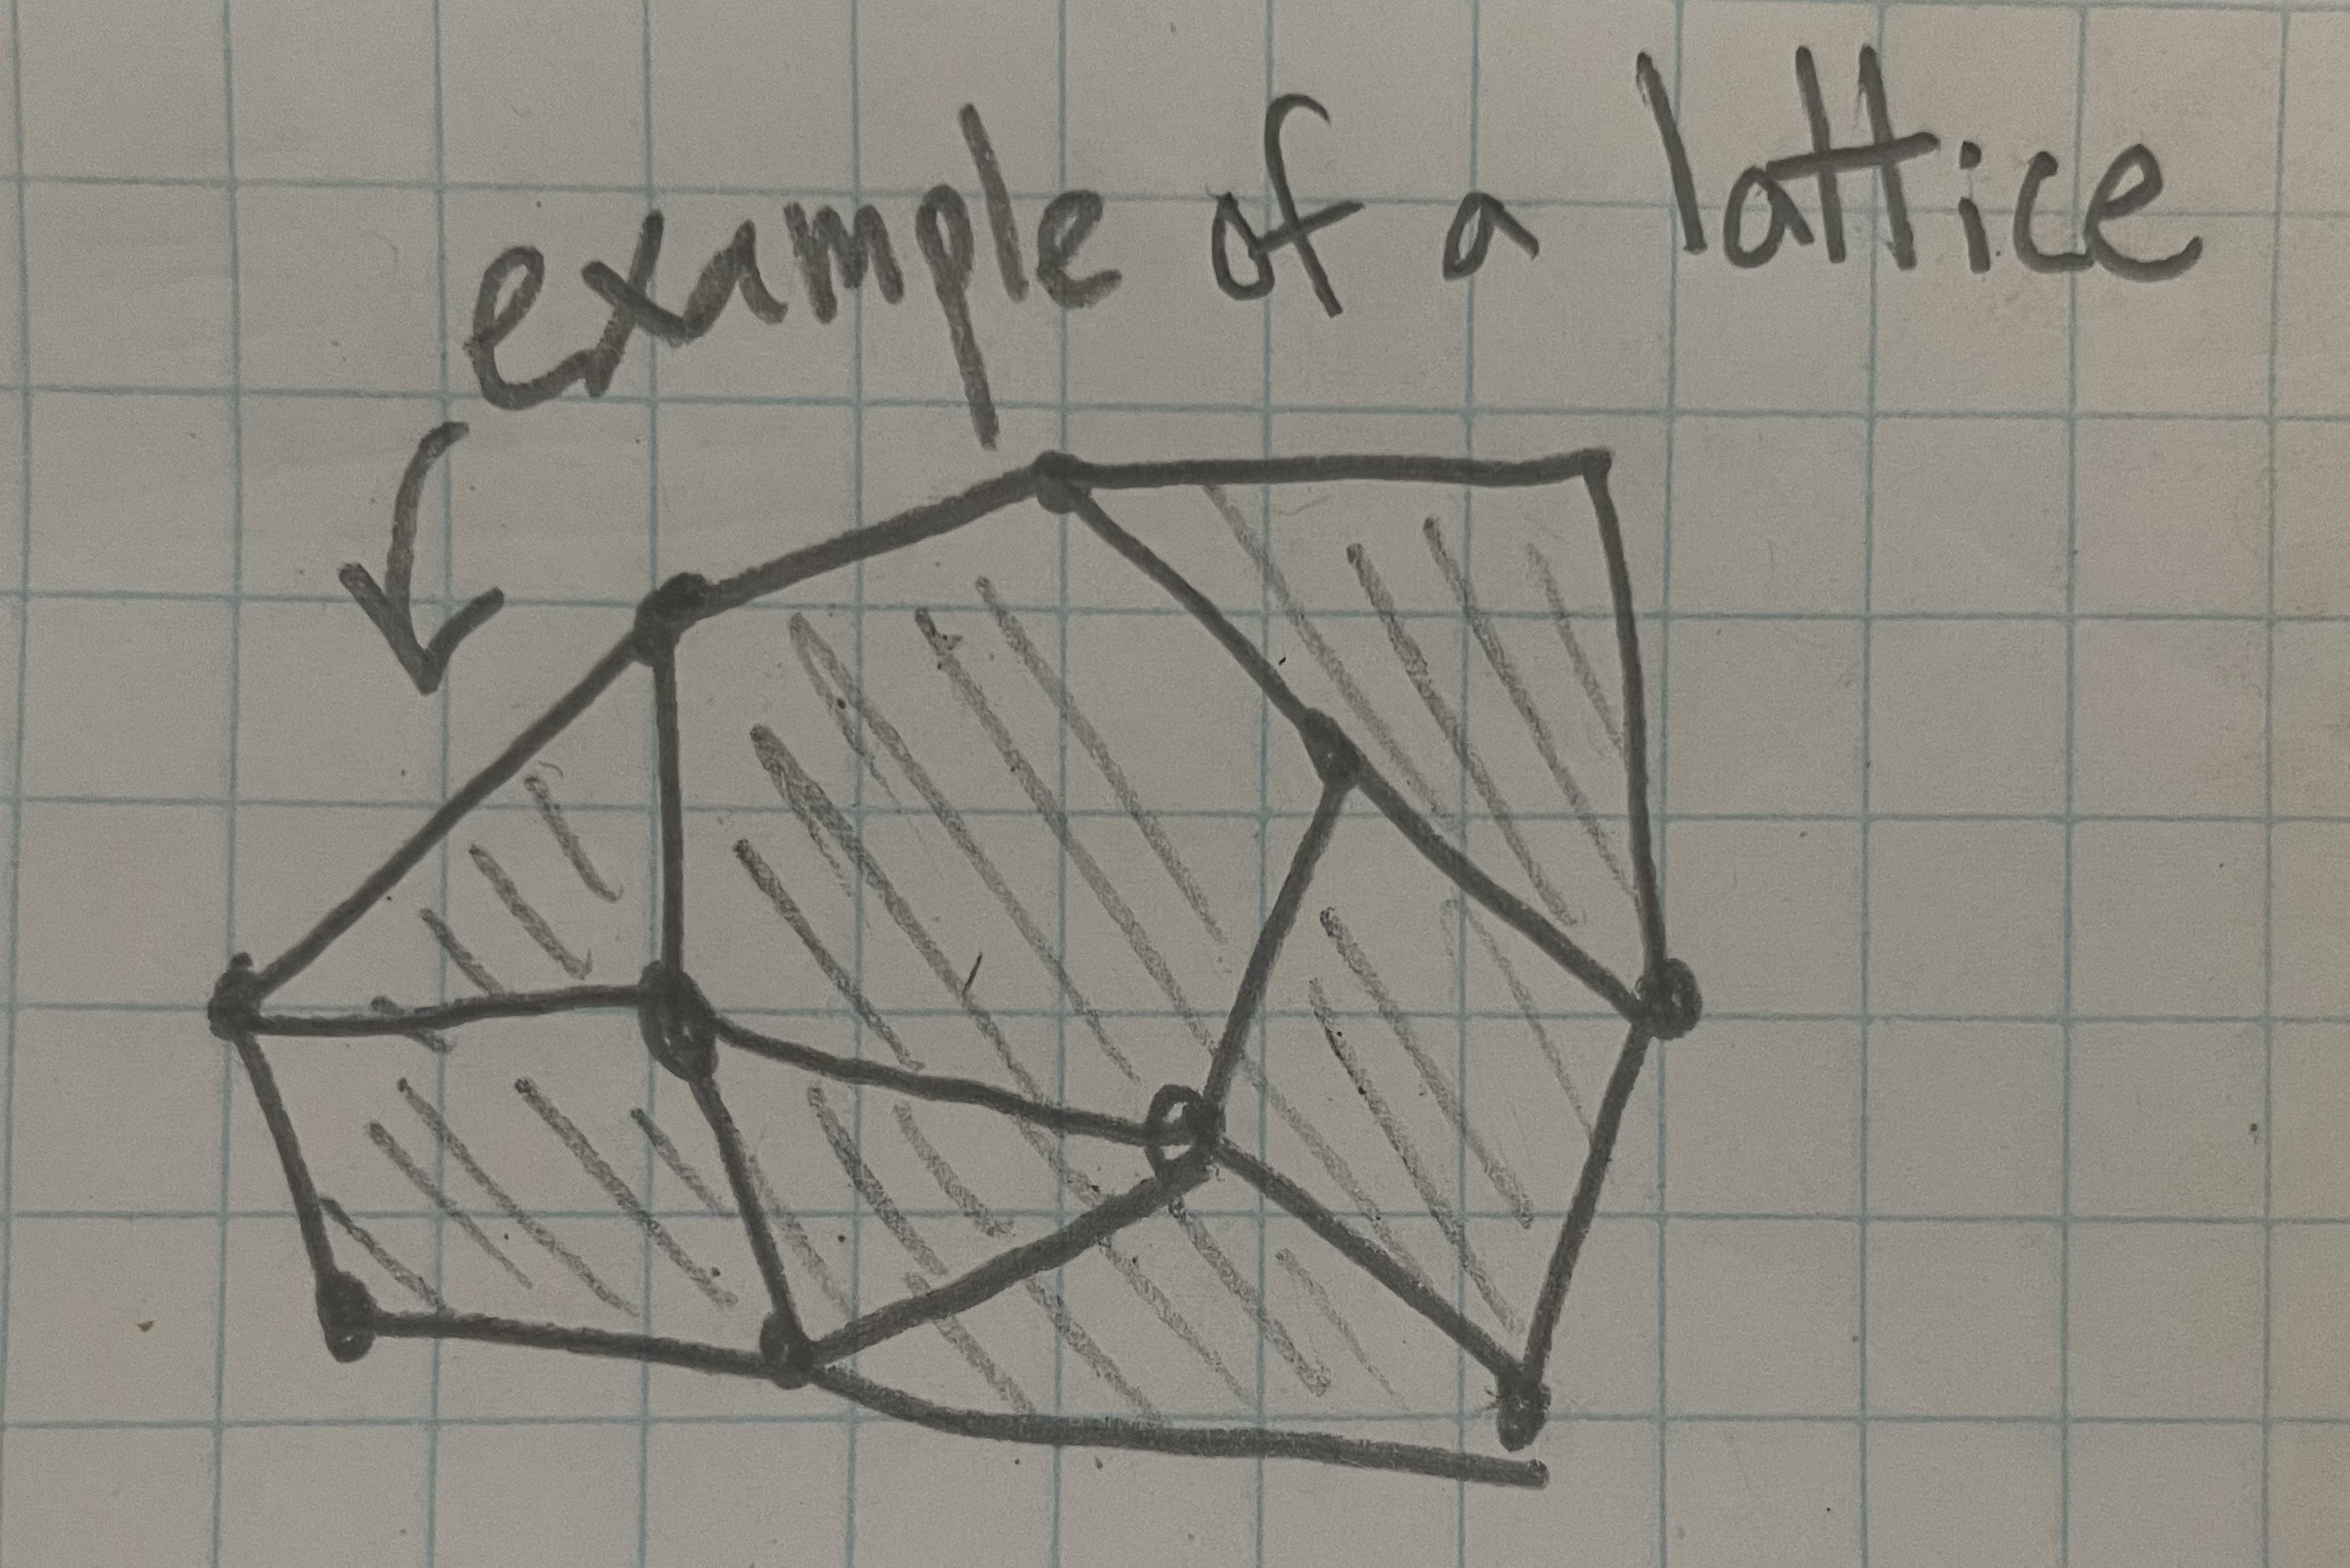
\includegraphics[scale=.04]{lattice-example}
\end{center}
\end{figure}

A lattice is a collection of vertices, edges, and faces connected in some way. To keep in line with the terminology common in topological quantum information, we refer to the faces of our lattices using the French term \textit{plaquette}. Formally, by lattice we mean ``simplicial 2-complex" though there is no need to go into details because we will never be dealing with the subtleties in the definition. Often times we will need to deal with \textit{directed} lattices. These are lattices in which every edge has a direction, which we represent as an arrow on that edge.

Before putting ordered media on a lattice, a good question is \textit{why} we would want to do this. There are two primary reasons. The first is that this will make this Hilbert spaces involved all finite dimensional. This is very important because we have only established quantum mechanics in the finite dimensional case, and working with the continuum limit can be highly complex. The second reason is that in practice, many of the systems physicists deal with are on lattices. For example, the chip of a quantum computer will store its information at finitely many sites, which can correspond to the vertices of some lattice. Many topological systems also arrise from materials which have crystal structures, which are modeled well by a lattice with atoms at the vertices and edges representing the geometry of the crystal.

The best setting for putting our ordered media on a lattice is by first putting on a torus. This helps for several reasons. Firstly, a torus is compact and hence it will add even more finiteness to the problem. Secondly, a torus has nontrivial topology which is useful for seeing the characteristic phenomina of topological order. Thirdly, a torus has no boundary, which helps because boundaries in topological order are subtle and require more work to describe. We denote the torus by $T^2$, and identify it with a square having its opposite sides glued:

\begin{figure}[h]
\begin{center}
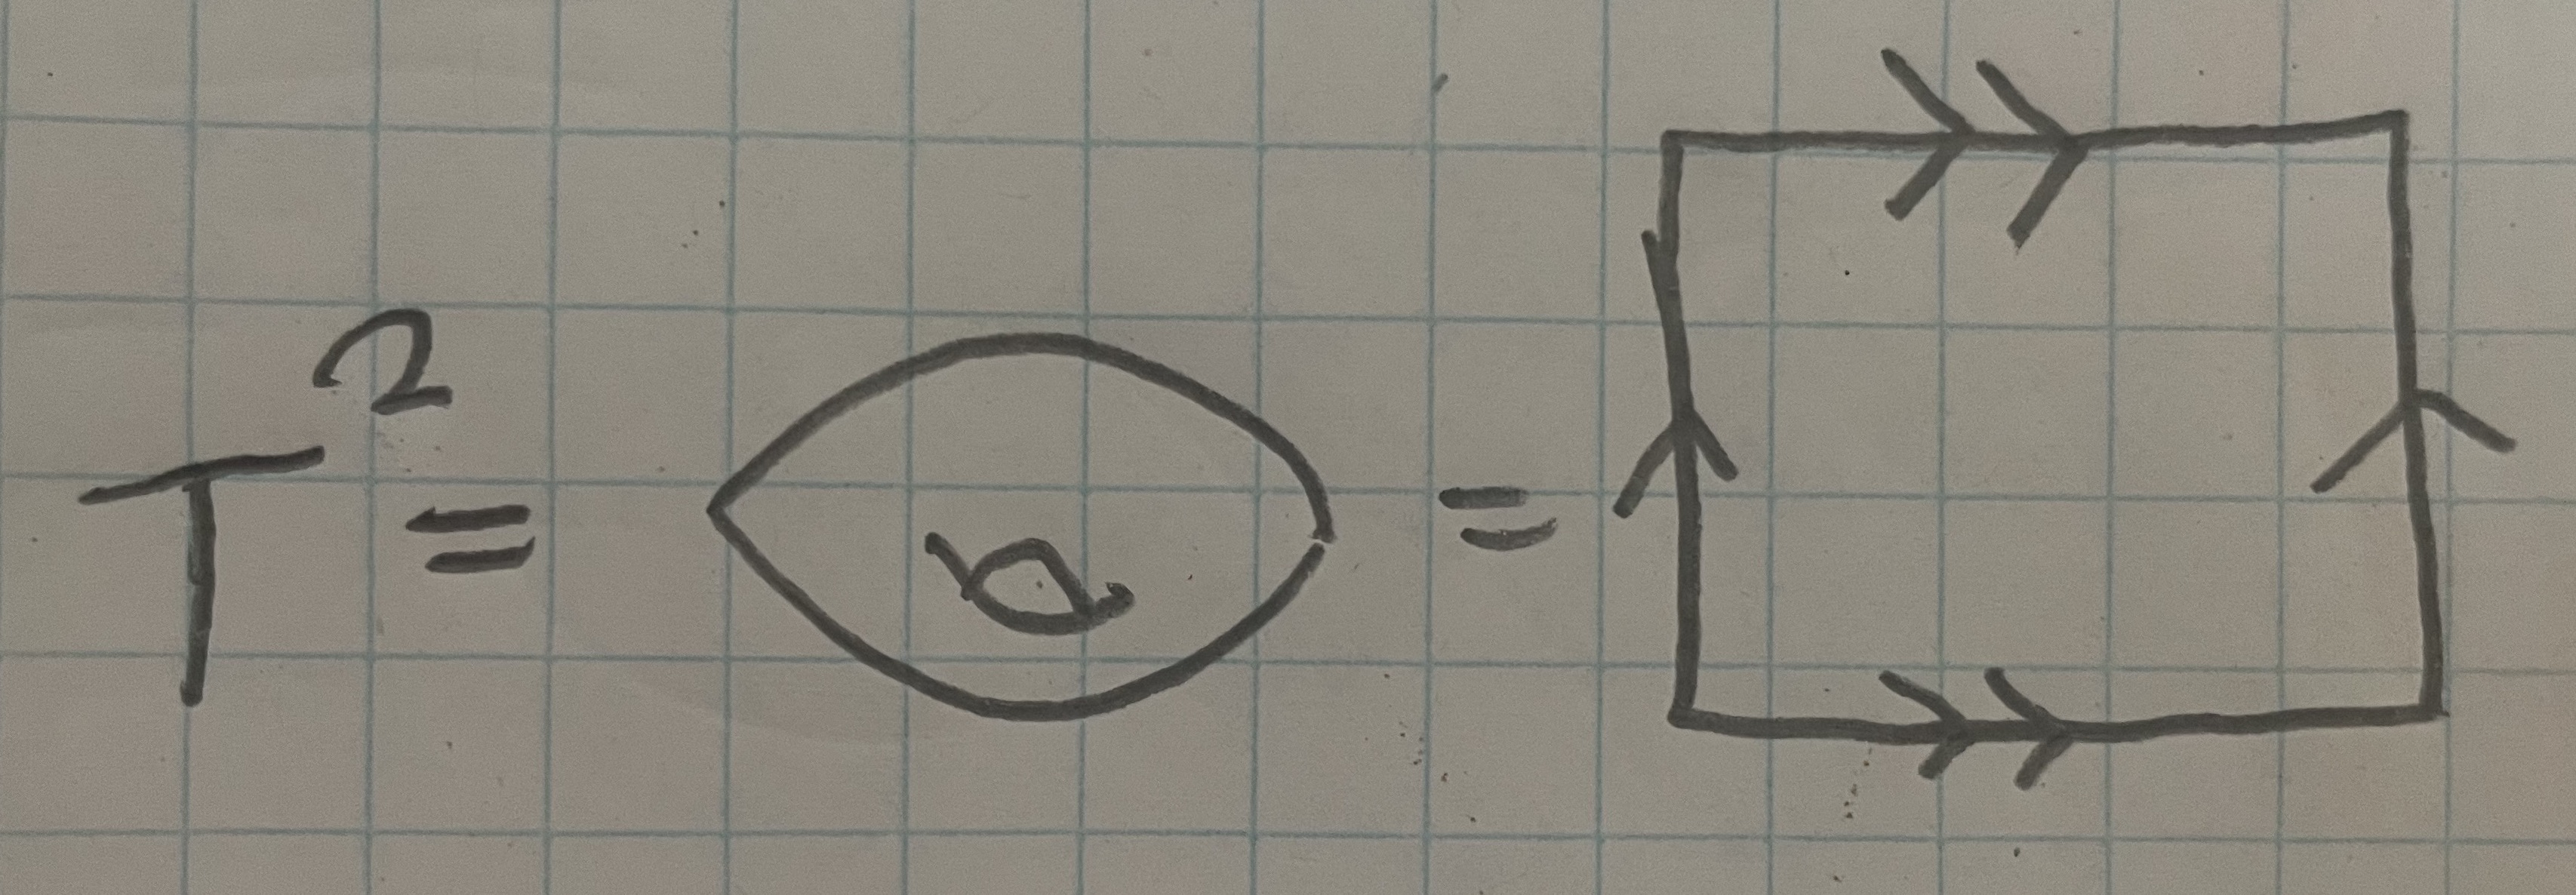
\includegraphics[scale=.04]{torus-definition}
\end{center}
\end{figure}

Ordered media on the torus corresponds to continuous maps $\phi: T^2\to M$ where $M$ is some fixed order space. The steps to transforming a state $\phi$ into a lattice version of itself go as follows:

\begin{enumerate}[Step $\text{1}$(a):]
\item Choose a directed lattice on the torus;
\item Choose a basepoint $m\in M$. Make \textit{local twists} around each vertex so that $\phi(v)=m$ for all vertices $v$ in the lattice.
\item On every edge, write down the winding number of $\phi$ along that edge, as an element of $\pi_1(M,m)$;
\item Forget $\phi$, and remember only the assignment of group elements in $\pi_1(M,m)$ to edges in the lattice.
\end{enumerate}

These steps deserve explanation. Step 1(a) is clear: we choose an arbitrary lattice on the torus. Typically we will choose the square lattice on the torus:

\begin{figure}[h]
\begin{center}
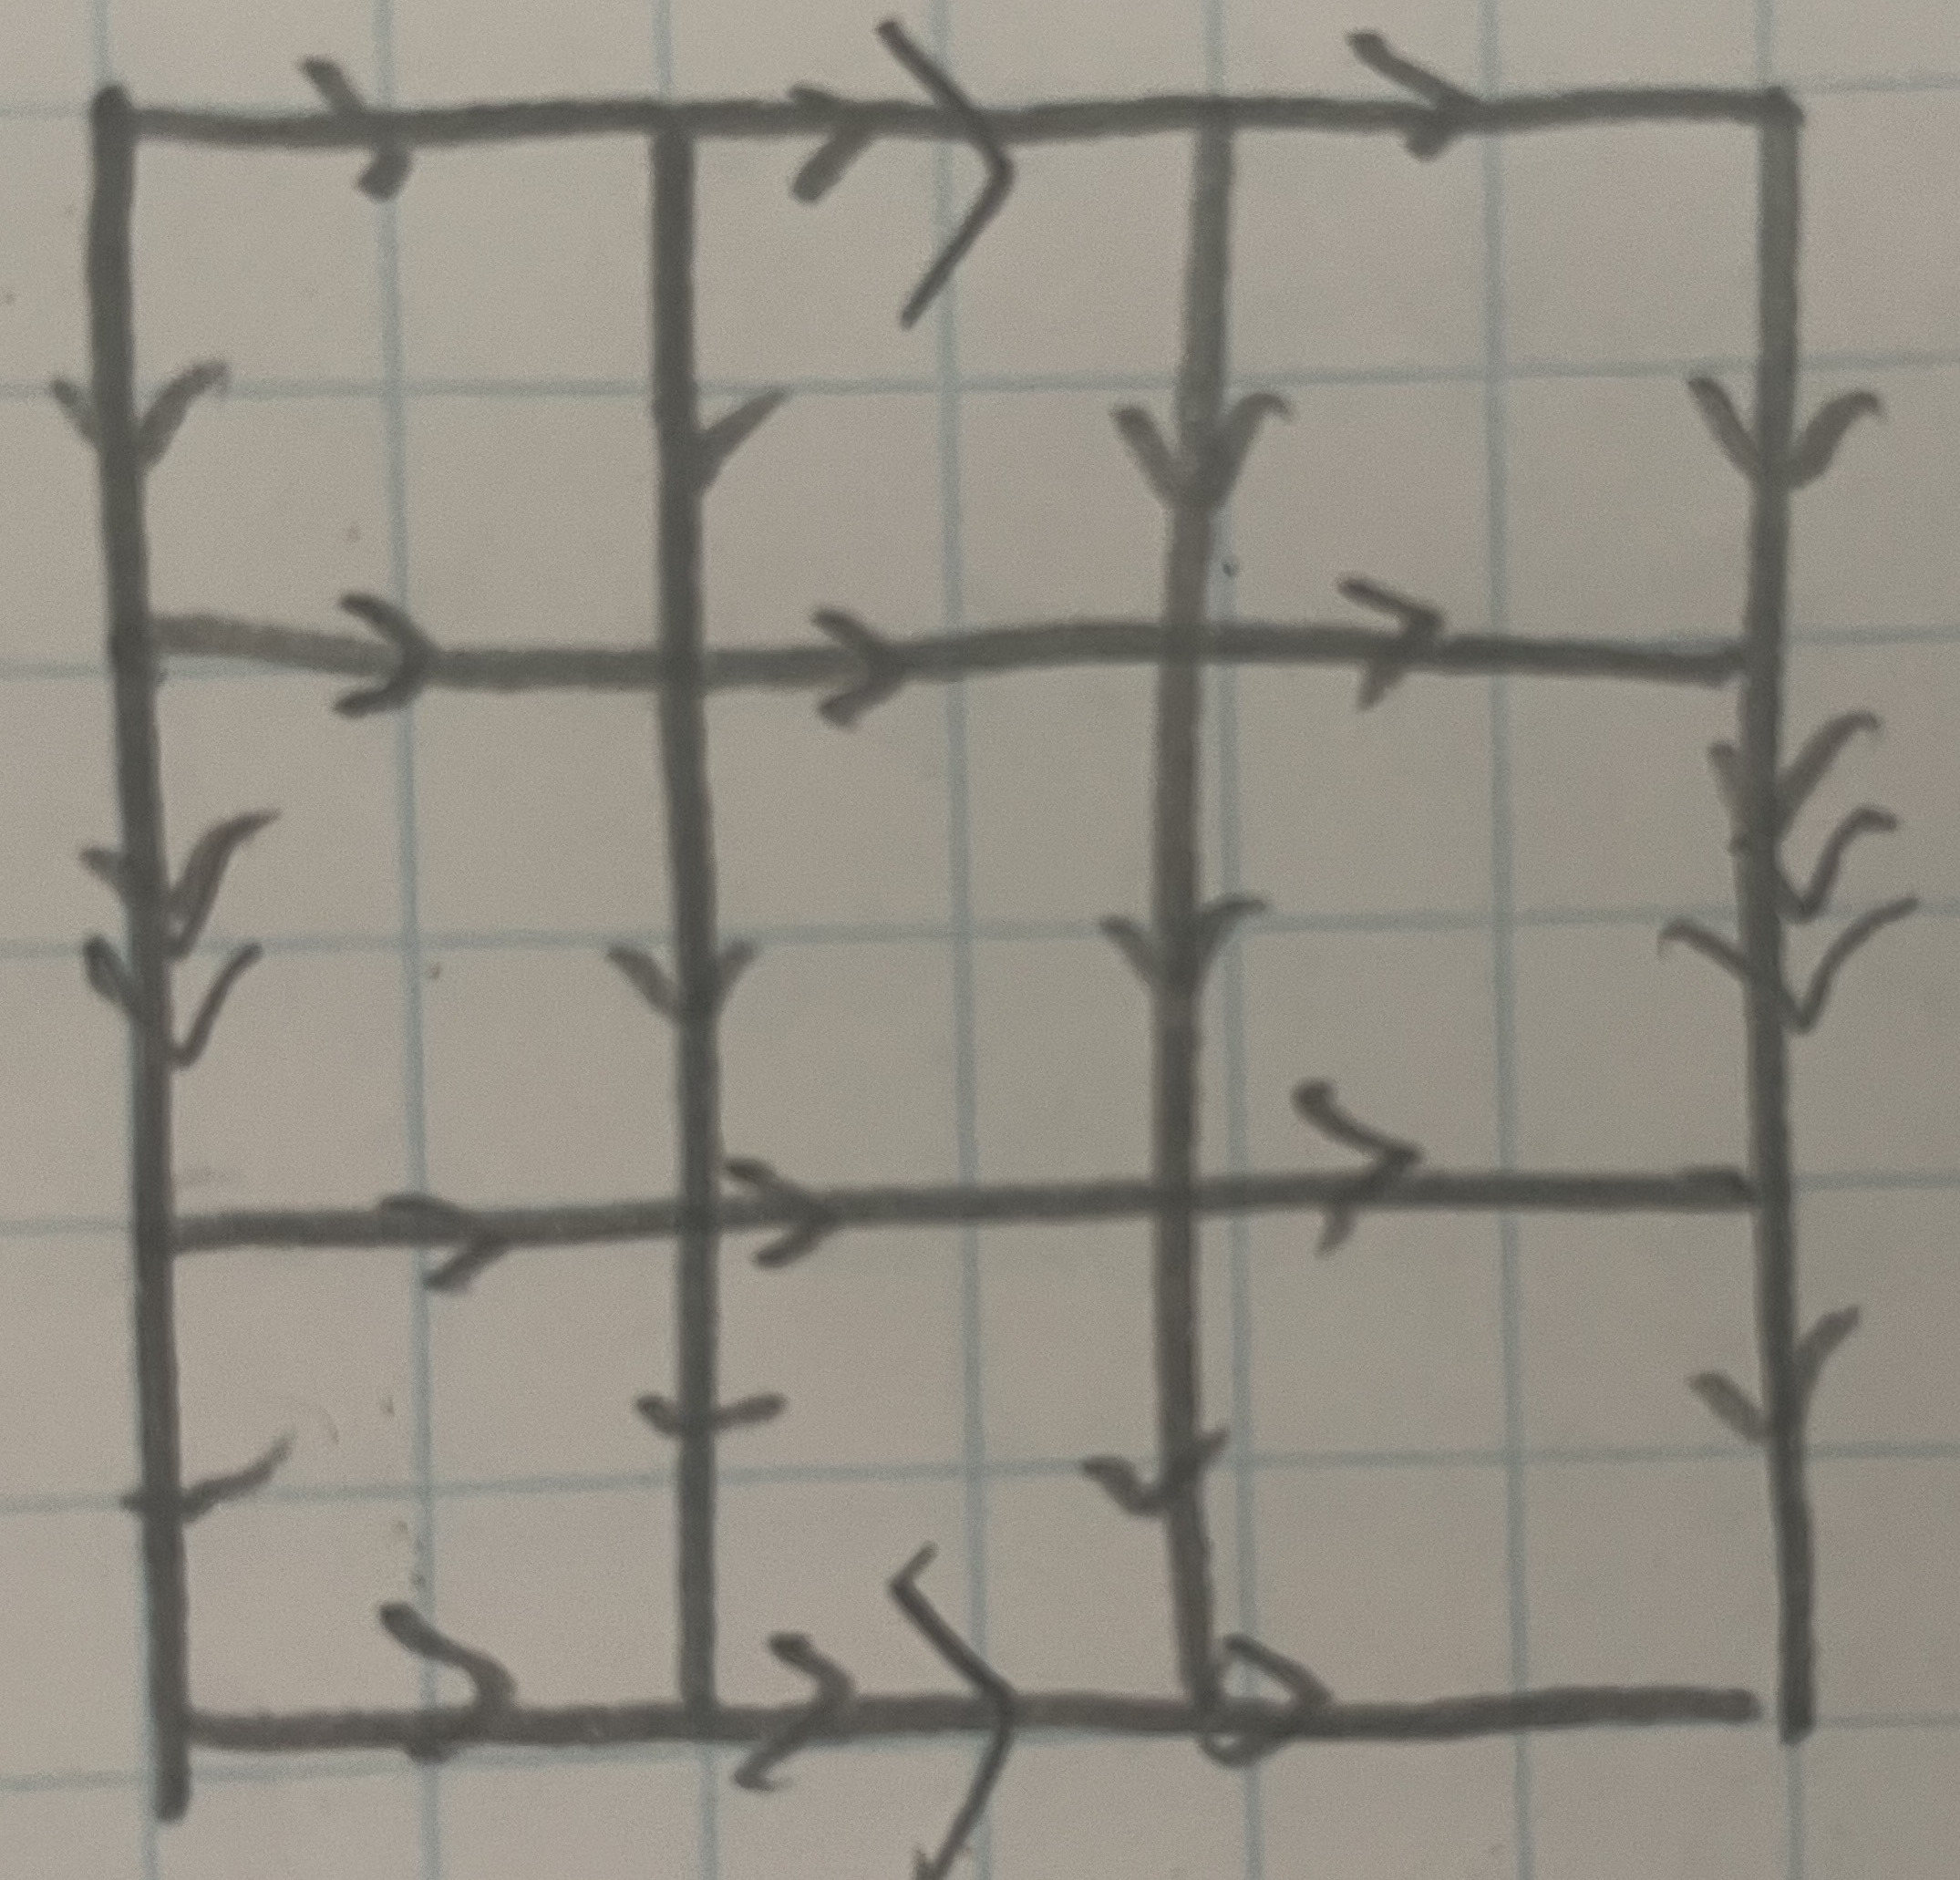
\includegraphics[scale=.04]{torus-lattice}
\end{center}
\end{figure}

Step 1(b) requires more explanation. The picture to imagine is that we take the state $\phi$ and twist its values in small neighborhoods around each vertex to enforce the condition $\phi(v)=m$. Formally, this means choosing another state $\tilde{\phi}$ such that $\tilde{\phi}(v)=m$ for every vertex $v$ of the lattice, and $\tilde{\phi}=\phi$ outside of some chosen small neighborhoods around each vertex. The fact that we can always choose such as state $\tilde{\phi}$ is a consequence of general mathematical principles in homotopy theory. Of course, different choices of $\tilde{\phi}$ will change the final result of our lattice encoding. However because any two choices of $\tilde{\phi}$ can only differ by local changes they can't be \textit{too} different, in a way we will quantify later in the subsection.

Step 1(c) is straightforward. Every edge can be thought of as a path. Pushing forward with $\phi$, this gives us a path in $M$. Since the edge starts and ends at vertices and $\phi$ sends all vertices to $m$, this means that the push forward of our edge gives a loop in $M$ based at $m$. Hence, it gives an element of $\pi_1(M,m)$. We can record this element and attach it as a piece of data associated to the edge.

Step 1(d) is entirely book keeping. It records the fact that we have successfully transformed our continuous data ($\phi:T^2\to M$) into discerete data (an assignement of group elements to edges in a lattice).

A worked example is shown below in the case that $M=S^1$ is the circle:

\begin{figure}[h]
\begin{center}
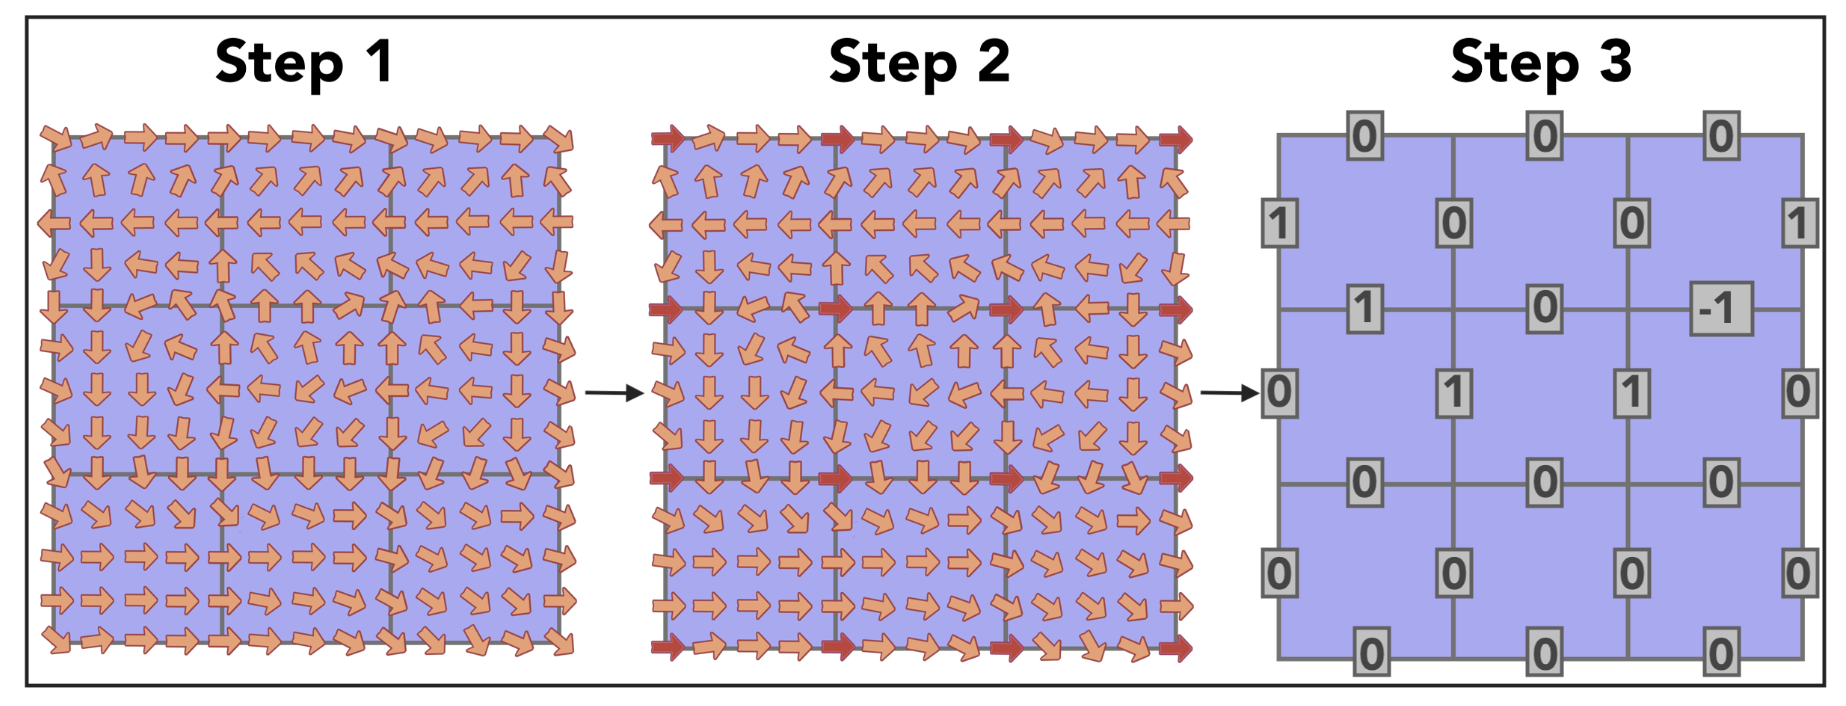
\includegraphics[scale=.3]{full-example}
\end{center}
\end{figure}

We now analyse our encoding of states in ordered media into assignements of group elements in $\pi_1(M,m)$ to edges in the lattice. The first fact from homotopy theory we will use is that these group elements determine the state $\phi$ exactly up to deformations localized within each face. Taking a limit of denser and denser lattices, this means that the group elements will specify $\phi$ up to increasingly local deformations. The intiution is that by taking an infinite lattice limit we should recover $\phi$ up to ``infinitely local deformations", i.e., we recover it exactly. In this way we did a good job with our lattice encoding.

We observe that not every assignement of group elements to edges appears in our construction. There are implicit conditions. In particular, imagine taking the product of the group elements on edges along some contractible loop, taking inverses appropriately so that all the arrows are pointing in the same direction. This product will be equal to the group element associated with the loop around this whole path. The winding number along any contractible path under a continuous map should be trivial. Hence, the product of these group elements should be trivial. In particular, given any plaquette, the ordered product of group elements along its edges should be zero:

\begin{figure}[h]
\begin{center}
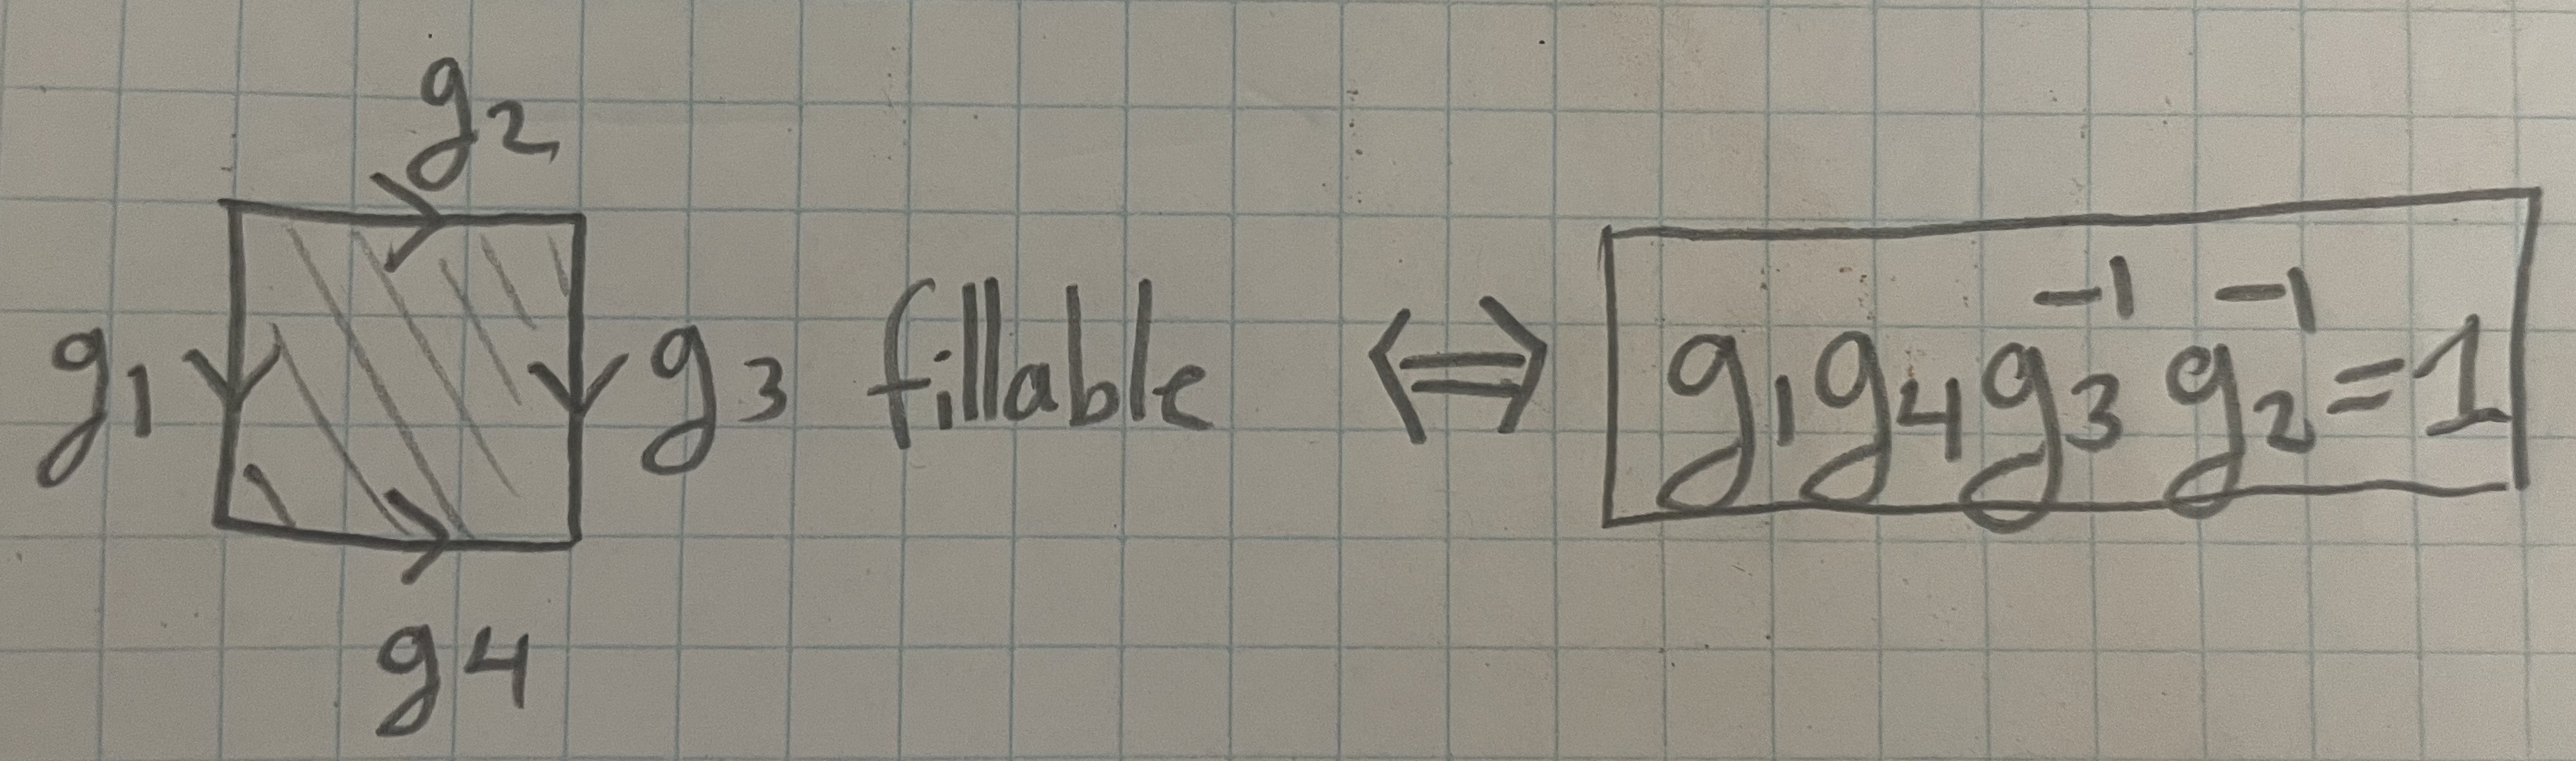
\includegraphics[scale=.06]{plaquette-rule}
\end{center}
\end{figure}

Moreover, \textit{any} coloring of the edges of the lattice by elements of $\pi_1(M,m)$ will come from some map $\phi$ so long as it satisfies the condition above. This is one of the key formulas of the theory. It is in a real sense a lattice version of the continuity condition, since it is \textit{equivalent} to the condition of continuity in the infinite lattice limit. This lattice version of continutity is called \textit{flatness}. Flatness conditions are the most common sort of compatibility conditions which appear when you have local degrees of freedom valued in some group, making this lattice situation very general.

The last thing do deal with in analysing our system is deformation. When analysing states in ordered media, a huge amount of our time was spent on performing continuous deformations. Topological information is defined to be information which is invariant under continuous deformation. What does this correspond to in the lattice model?

Suppose we are given an ordered media state $\phi$ and its corresponding lattice coloring. If we deform $\phi$ in some small neighborhood within a face, this will not change the values along the edges and hence will not change the coloring. If we deform $\phi$ in some small neighborhood around the interior of some edge this also won't change the coloring, because this will correspond to deforming the loop in $M$ induced by going along that edge, and elements of the fundamental group are invariant under deformations of this sort. Another way of seeing that the coloring can't change is that flatness must be preserved - if the group element on the deformed edge changed, it would ruin flatness on the faces it bounds.

Finally, we can consider deforming $\phi$ around some vertex. This certainly \textit{can} impact the coloring. An easy way to compute how it must impact the coloring is by using the fact that the flatness condition must be preserved. Suppose that an incoming edge labled by $g_1$ changes to $g_1 g$ after the deformation. Enforcing flatness along all of the faces touching the vertex allows one to conclude that all incoming edges $g_k$ will get changed to $g_k g$, and all outgoing edges $g_k$ will get changed to $g^{-1}g_k$, as shown below:

\begin{figure}[h]
\begin{center}
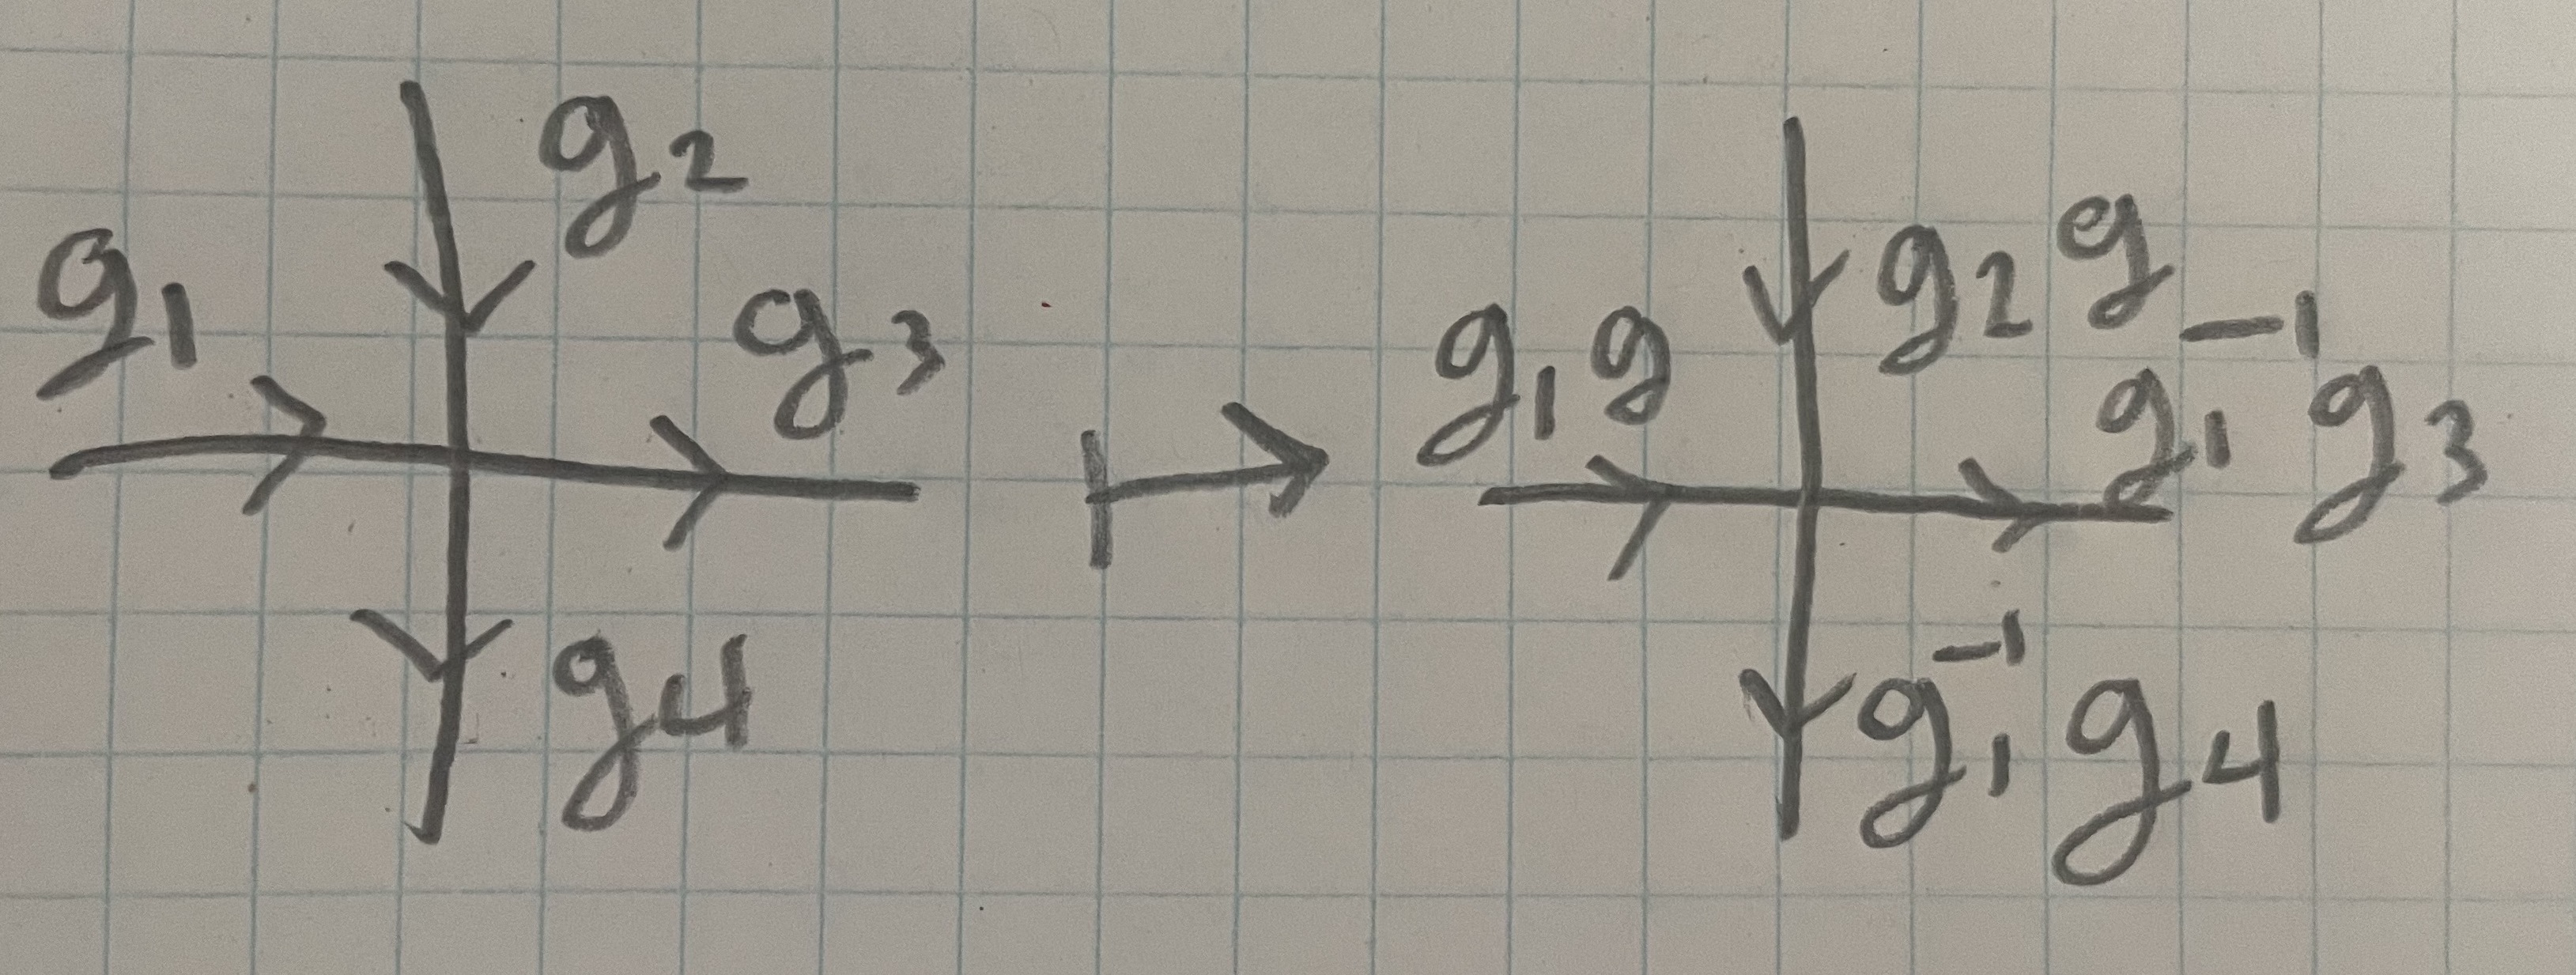
\includegraphics[scale=.04]{gauge-transformation}
\end{center}
\end{figure}

Another way of seeing this result is by anlysing what a deformation of $\phi$ does. The value $\phi(v)$ can move along some loop, starting and ending at $m$. This loop induces some element of the fundamental group, $g\in \pi_1(M,m)$. Performing this deformation exactly acts by precomposing/postcomposing the adject edges with $g$/ $g^{-1}$ accordingly. We can see below a concrete example for $G=S^{1}$:

\begin{figure}[h]
\begin{center}
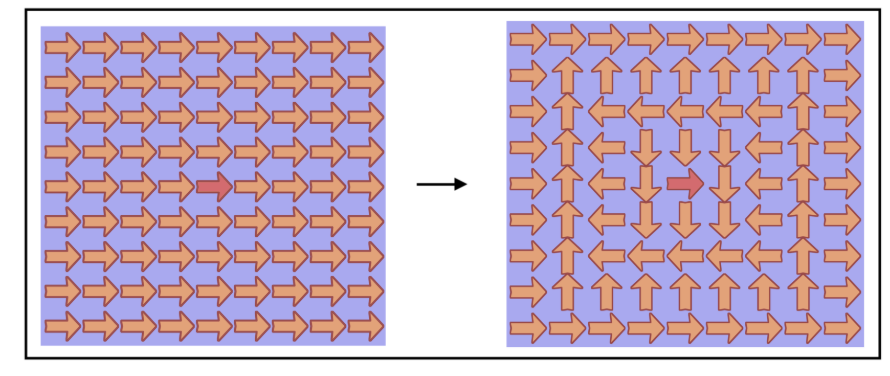
\includegraphics[scale=.45]{twisting}
\end{center}
\end{figure}

Hence, we have a picture for ordered media on the lattice: states correspond to flat colorings of elements of $\pi_1(M,m)$ on a fixed lattice, and continuous deformations correspond to certain vertex actions by elements of $\pi_1(M,m)$.

\subsubsection{From ordered media to gauge theory}

In the previous subsection we showed how to put ordered media on a lattice. In this section we show how to make it quantum, turning it from a classical field theory to a quantum gauge theory. The idea of this jump is as follows. In Section [ref] we obtained an equivalence

$$
\left(\substack{\text{topological information}\\ \text{in ordered media}}\right)=\left(\text{states}\right)/\left(\substack{\text{continuous} \\ \text{deformation}}\right).
$$

It is neccecary to mod out by continuous deformation because there is topoloigcal information in states, but also local degrees of freedom. For instance, the group element assigned to any indivudal edge in ordered media on a lattice can be changed by a gauge transformation and hence is not topologically invariant. The idea of going from ordered media to gauge theory is as follows: gauge theory is what results from ordered media when quantum fluxtuations become so strong that local degrees of freedom are completely washed out and only the topology remains.

The fluxtuations are quantum because we will imagine that our states will evolve in such a way that they are in a superposition of gauge transformations having been applied and not having been applied. Our states in gauge theory will be \textit{equal superpositions over all possible deformations} of a given state. In this way, we are using quantum mechanics as a physical mechanism for quotients. Equivalence classes under deformation will be physically realized as equal superpositions over all possible representatives.

This can all be made completely rigorous. Choose a lattice on the torus, an order space $M$, and a basepoint $m$. We define a Hilbert space

$$\NN=\bigotimes_{\text{edges}}\CC[G].$$

We canonically identify the standard basis of $\NN$ with $G$-colorings of the lattice. Let $C$ be an equivalence class of flat $G$-colorings of $\NN$ up to gauge transformations. There is a corresponding state

$$\ket{C}=\sum_{\gamma \in C}\frac{1}{\sqrt{|C|}}\ket{\gamma}.$$

This state is a normalized equal superposition of representatives of $C$. This defines a sub-Hilbert space

$$\Cc=\text{span}\left\{\left.\ket{C}\right| C\in \text{(flat $G$-colorings)}/\text{(gauge transformations)}\right\}.$$

This Hilbert space $\Cc$ stores the information in our gauge theory.

So far our system is relatively trivial - it is just a Hilbert space, with no Hamiltonian. We connect it back to our original picture of topological order. The space $\Cc$ is the collection of ground states in a topologically ordered system. Above it there is a whole spectrum of other states. This fuller picture with a Hamiltonian adds all of the subtlety and intrigue to the system.

In particular, we observed in Chapter [ref] section [ref] we observed the importants of quasiparticles in ordered media. These formed the heart of our information processing. Similarly, in gauge theory there will be quasiparticles as well, which appear as anyons higher up in the spectrum of the Hamiltonian. Some of these anyons correspond to the classical quasiparticles in ordered media, but other anyons are entirely new features of the system which did not exist before. We will analyse all this in more in the subsection that follows.

\subsubsection{Kitaev quantum double model}

[WORK: not sure if this is readable to someone who skipped the first two sections, but it should be. Something to keep an eye on.]

[WORK: Use $\D(G)$ as notation for the doubled quantum order associated to $G$.]

In this section we will give the Hamiltonian formulation of discrete gauge theory. Seeing as we have moved passed ordered media, we will no longer be working with order spaces and base points. Instead, we will choose an abstract finite group $G$ which replaces $\pi_1(M,m)$. The general picture for creating our Hamiltonian is simple, and follows a very general pattern in quantum theory: instead of enforcing properties rigidly as conditions, we will enforce them enforce properties energetically as terms in a Hamiltonian. The formulation we give below is known as the \textit{Kitaev quantum double model of discrete gauge theory}. It was introduced in Kitaev's seminimal paper on topological quantum information [ref]. It has been studied extensively in the literature by many authors [add more refs].

Choose a directed lattice on the torus. Let

$$\NN=\bigotimes_{\text{edges}}\CC[G]$$

be the HIlbert space of our quantum system. The space $\NN$ has a canonical basis given by $\prod_{\text{edges}}G$, which we  identify with $G$-colorings of the lattice. Given a $G$-coloring $\gamma$, we will denote the corresponding state in $\NN$ by $\ket{\gamma}$. For every plaquette $p$ in the lattice, we define an operator on $\NN$ by

$$B_p\ket{\gamma}=
\begin{cases}
\ket{\gamma} & \gamma \text{ flat at }p\\
0 & \text{otherwise}.
\end{cases}$$

We observe immediately that

$$\sum_{\text{plaquettes }p}(1-B_p)\ket{\gamma}=0 \iff \ket{\gamma} \text{ is flat.}$$

It is in this way that we can enforce properties energetically by adding them as terms to a Hamiltonian. If we chose the Hamiltonian to be $\sum_{\text{plaquettes }p}(1-B_p)$, then the lowest energy eigenspace would exactly correspond to the space spanned by flat $G$-colorings. For every vertex $v$ and group element $g\in G$, we define an operator on $\NN$ by

$$A_{v,g}\ket{\gamma}=\ket{\gamma \text{ acted on by the $g$ gauge action at $v$}}.$$

For any $\ket{\psi}\in \NN$, we call $\ket{\psi}$ \textit{gauge invariant at $v$} if $A_{v,g}\ket{\psi}=\ket{\psi}$ for all $g\in G$. We call $\ket{\psi}$ gauge invariant if it is gauge invariant at $v$ for all vertices $v$. We define

$$A_v=\frac{1}{|G|}\sum_{g\in G}A_{v,g}.$$

We define the Hamiltonian of our system to be

$$H=\sum_{\text{vertices $v$}}(I-A_v)+\sum_{\text{plaquettes $p$}}(I-B_p)$$

where $I$ is the identity operator. We summarize the basic properties of this Hamiltonian below:

\begin{proposition} The following properties of the Kitaev quantum double Hamiltonian hold:

\begin{enumerate}[(a)]
\item The operators $A_v$, $B_p$, and $H$ are Hermitian for all vertices $v$ and plaquettes $p$;
\item The formula $A_{v,g}^{\dagger}=A_{v,-g}$ holds for all vertices $v$ and $g\in G$;
\item All of the operators in the set $\{A_v,B_p\}_{v\in \text{vertices}, p\in \text{plaquettes}}$ commute with every other operator in the set;
\item The eigenstates of $H$ are simultaneous eigenstates of the operators $A_v$, $B_p$;
\item The eigenvalues of the $A_v,B_p$ are all $0$ or $1$;
\item The lowest eigenvalue of $H$ is $0$, and the $0$-eigenspace of $H$ is

$$\Cc=\text{span}\left\{\left.\ket{C}\right| C\in \text{(flat $G$-colorings)}/\text{(gauge transformations)}\right\}.$$

where for we define the ket

$$\ket{C}=\sum_{\gamma \in C}\frac{1}{\sqrt{|C|}}\ket{\gamma}$$

for any equivalence class $C$ of $G$-colorings of the lattice up to gauge transformations.

\end{enumerate}
\end{proposition}
\begin{proof}.[WORK: do proof]
\end{proof}

In particular, the above proposition tells us exactly that we have acheived our goal of realizing a Hamiltonian whose ground states capture the topological information in a lattice-version of ordered media.  The term ``double" in the Kitaev quantum double model refers to the fact that there are two families of terms in $H$ - one family of type $A_v$ and one family of type $B_p$. We can readily compute the dimension of the ground space as follows:

\begin{proposition} Choose a vertex $v$ in the lattice. Every $G$-coloring of the lattice induces an assignment of lattice loops on the torus based at $v$ to elements of $G$, based on taking the oriented winding number along that loop relative to the coloring. This restricts to a map

$$(\text{flat $G$-colorings})\xrightarrow{}\Hom(\pi_1(T^2,v), G)$$

where $\Hom(\cdot,\cdot)$ denotes the space of group homomorphisms between two groups. Any two flat $G$-colorings which differ by gauge transformations will induce the same map in $\Hom(\pi_1(T^2,v), G)$, up to global conjugation by an element of $G$. This induces a bijection

$$(\text{flat $G$-colorings})/(\text{gauge transformations})\xrightarrow{}\Hom(\pi_1(T^2,v), G)/\left(\substack{\text{simultaneous} \\ \text{conjugation}}\right).$$

The set of vectors ${\ket{C}}_{C\in (\text{flat $G$-colorings})/(\text{gauge transformations})}$ is linearly independent. Hence, there is a canonical isomorphism

$$\Cc \xrightarrow{}\CC[\Hom(\pi_1(T^2,v), G)/\left(\substack{\text{simultaneous} \\ \text{conjugation}}\right)]$$

given by taking winding numbers.
\end{proposition}
\begin{proof}.[WORK: give proof]
\end{proof}

The final step in using the above formula is to compute the fundamental group of the torus:

\begin{proposition} $\pi_1(T^2,v)\cong \ZZ^2$ for any vertex $v$. The two loops shown below are generators for $\pi_1(T^2,v)$:

\begin{figure}[h]
\begin{center}
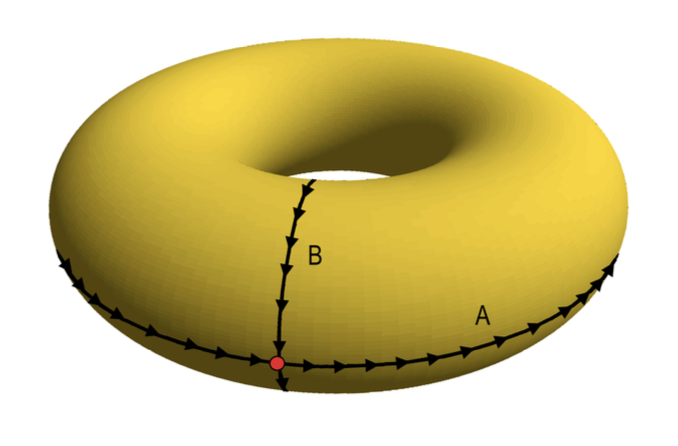
\includegraphics[scale=.3]{torus}
\end{center}
\end{figure}

\end{proposition}
\begin{proof}.[WORK: proof]
\end{proof}

One last observation to make about this ground space is that its ground states really are globally different:

\begin{proposition} Let $L$ be length of the shortest non-contractible loop on the lattice. Let $\gamma_0,\gamma_1$ be non-gauge equivalent flat $G$-colorings of the lattice. There are at least $L$ edges at which $\gamma_0$ and $\gamma_1$ assign different values.
\end{proposition} 
\begin{proof}.[WORK: do proof]
\end{proof}

In particular, if we choose the square lattice on the torus, then the length $L$ of the shortest non-contractible loop is obvioulsy a good measure of linear system size. Proposition [ref] tells us that the number of local changes requires to go from one ground state to another is on the order of $L$. This is exactly the sort of condition we needed in Section [ref] to conclude topological protection in the ground states. Of course, the smallest non-zero eigenvalue of $H$ is at least $1$, which is bounded away from zero and hence there is a system-size independent gap between the ground states and the other states. Hence, we see that $H$ is a good topologically ordered Hamiltonian. 

The excited states of $H$ will be described localized excitations with quasiparticle behavior. Given a state $\ket{\psi}\in \NN$, we will say that a state has an \textit{anyon at vertex $v$} if $A_v\ket{\psi}=0$ and we will say that is \textit{unnoccupied at $p$} if $A_v\ket{\psi}=1$. We say that $\ket{\psi}$ has an \textit{anyon at plaquette $p$} if $B_p\ket{\psi}=0$ and that it is \textit{unnocupied at $p$} if $B_p\ket{\psi}=1$. By Proposition [ref], every energy eigensate is either occupied or unoccupied at every vertex/plaquette. The regions in which $\ket{\psi}$ is unnoccupied are all essentially identical, leading to a homogenous bulk. The sites at which $\ket{\psi}$ is occupied are different, and behave as quasiparticles. We will define operators which move these excitations around.

We think of these anyons as being localized within faces or within arbitrarily small regions around vertices depending on whether they are vertex-type or plaquette-type. We will find that the states of $H$ can be almost entirely described by anyons and their behavior .

[WORK: Add something about local indistinguishability of ground states - reinforce this ``homogenous bulk" idea.

More than this, it is important to note that earlier we are giving a rigorous definition of topological order. It is not immediately obvious that the KQDM satisfies this definition. This is the main content of the paper \cite{cui2020kitaev}. Should I include a proof? At the very least there should be some mention of how this fits into the definition.]

[WORK: Maybe also reinforce that this could be done on \textit{any manifold}, and the gound states would be the same? ]

\subsection{The toric code}

\subsubsection{Exact solution}

In this section we move on to analyzing the Kitaev quantum double model for $G=\ZZ_2$, which is known as the \textit{toric code}. The name toric code comes from the fact that the toric code was first introduced as an error correcting code, and was only later recast as a topologically ordered system [refs]. The toric code is still the basis for many of the most popular error correcting codes [refs]. In a real sense the toric code is the simplest nontrivial topological order. It is a fantastic example which demonstrates almost all of the phenomina of topological order with relatively little work involved. The toric code, and more generally $\ZZ_2$ discrete gauge theories, can be found in all sorts of systems such as [WORK: give examples]. 

We describe the model now. Because $G=\ZZ_2$ is abelian, we will switch to additive notation for our group operation. We choose a \textit{non-oriented} lattice structure on the torus. This lattice does not need to be oriented because changing the direction of edges in the lattice corresponds to taking inverses, and $g=g^{-1}$ for every element $g\in \ZZ_2$. We define

$$\NN = \bigotimes_{\text{edges}}\CC[\ZZ_2]=\bigotimes_{\text{edges}}\CC^2.$$

Here, we identify $\CC[\ZZ_2]$ with $\CC^2$ for convenience, endowing $\CC^2$ with a canonical basis $\{\ket{0},\ket{1}\}$. We call $\CC^2$ a \textit{qubit}, in analogy to ``bits" for classical computing. It is a standard two-level quantum system. Most quantum computers are based on qubits, which makes the toric code especially accessable to practical implementation as an error correcting code. The definition of the Hilbert space $\NN$ can be summarized as putting a qubit on every edge of the lattice. The Hamiltonian is

$$H=\sum_{\text{vertices }v}(1-A_v)+\sum_{\text{plaquettes }p}(1-B_p).$$

We unpack the general definitions of $A_v$ and $B_p$ for the toric code. The operator $A_{v,0}$ is the identity. The operator $A_{v,1}$ acts by a gauge transformation,

\begin{figure}[h]
\begin{center}
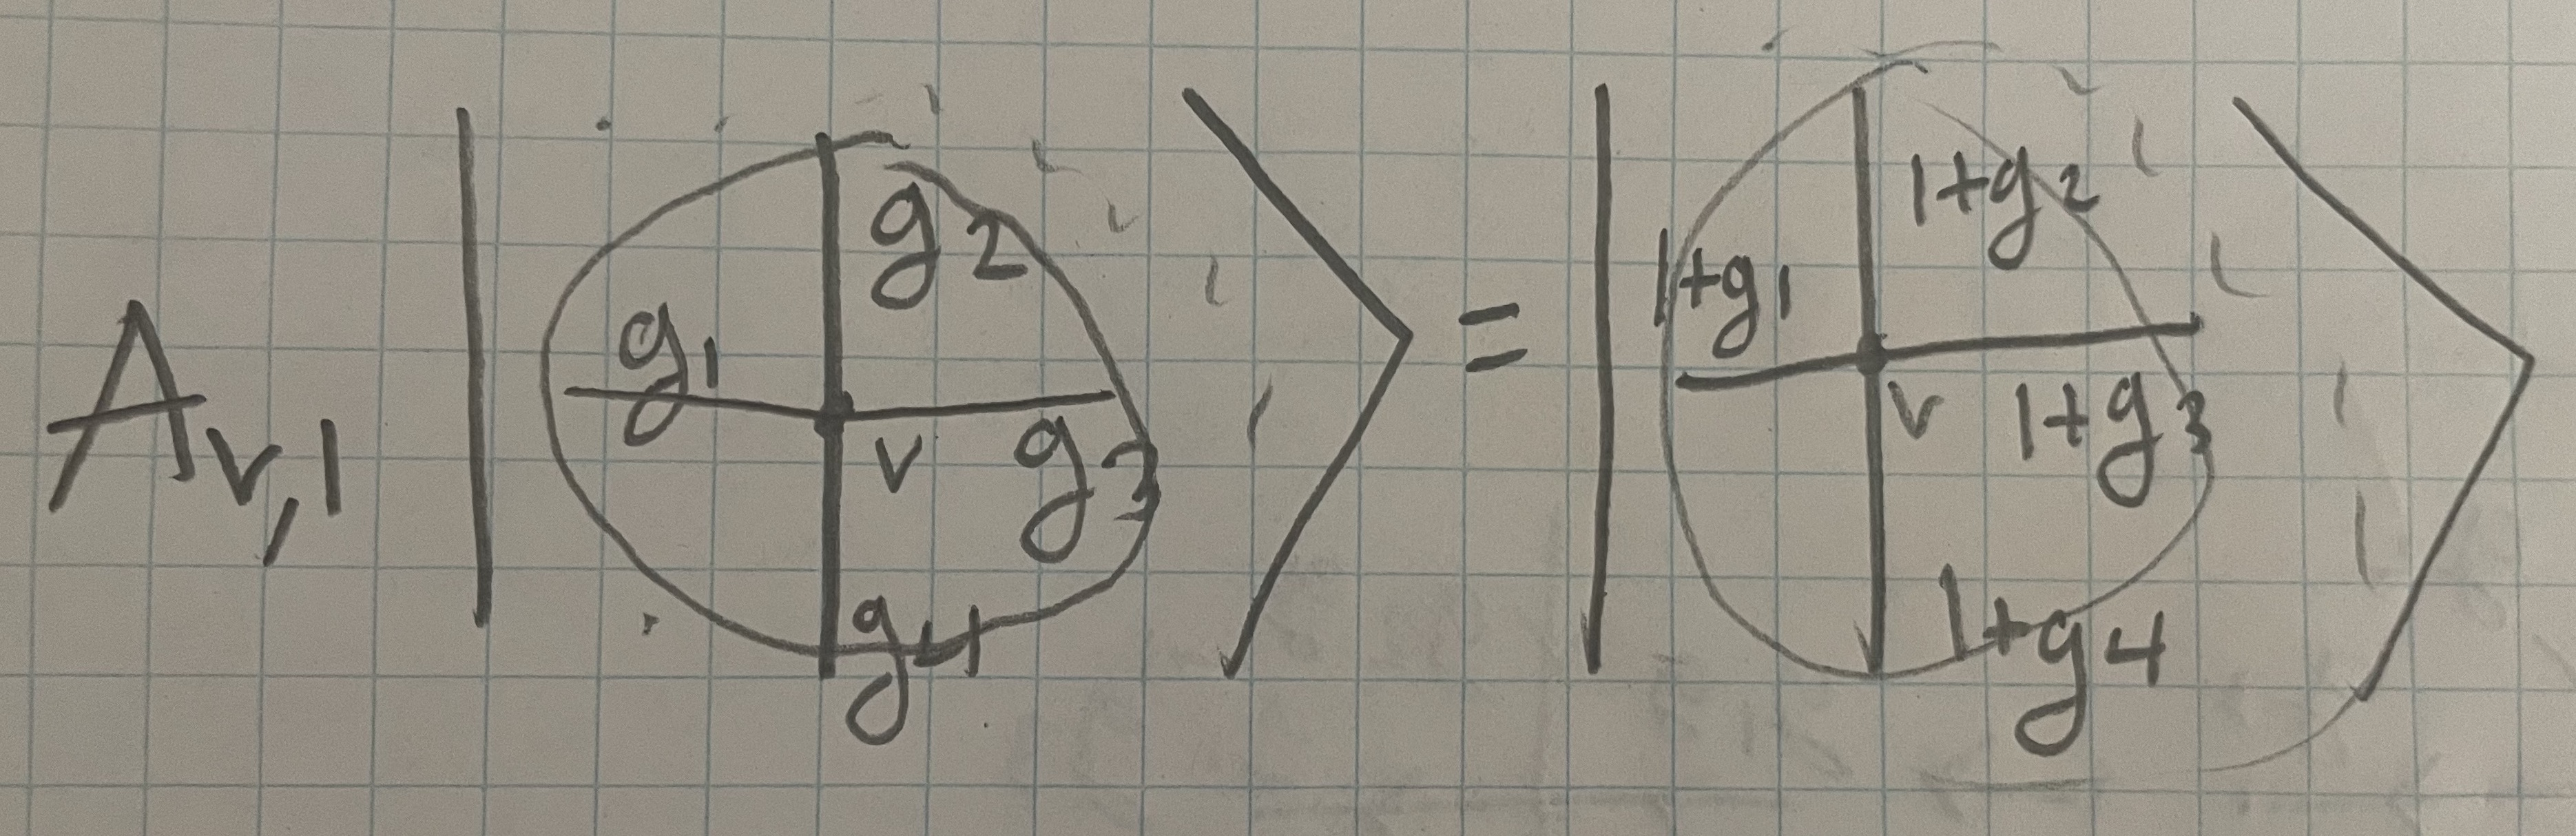
\includegraphics[scale=.04]{Av-gauge-action}
\end{center}
\end{figure}

Defining

\begin{align*}
\sigma_X:\CC^2&\xrightarrow{}\CC^2\\
\ket{0}&\mapsto \ket{1}\\
\ket{1}&\mapsto \ket{0}
\end{align*}

we thus find that

\begin{align*}
A_{v,1}=\bigotimes_{\substack{\text{edges} \\ \text{touching }v}}\sigma_X, && A_v=\frac{1}{2}\left(I + A_{v,1}\right).
\end{align*}

Moving on to $B_p$, we recall that

\begin{figure}[h]
\begin{center}
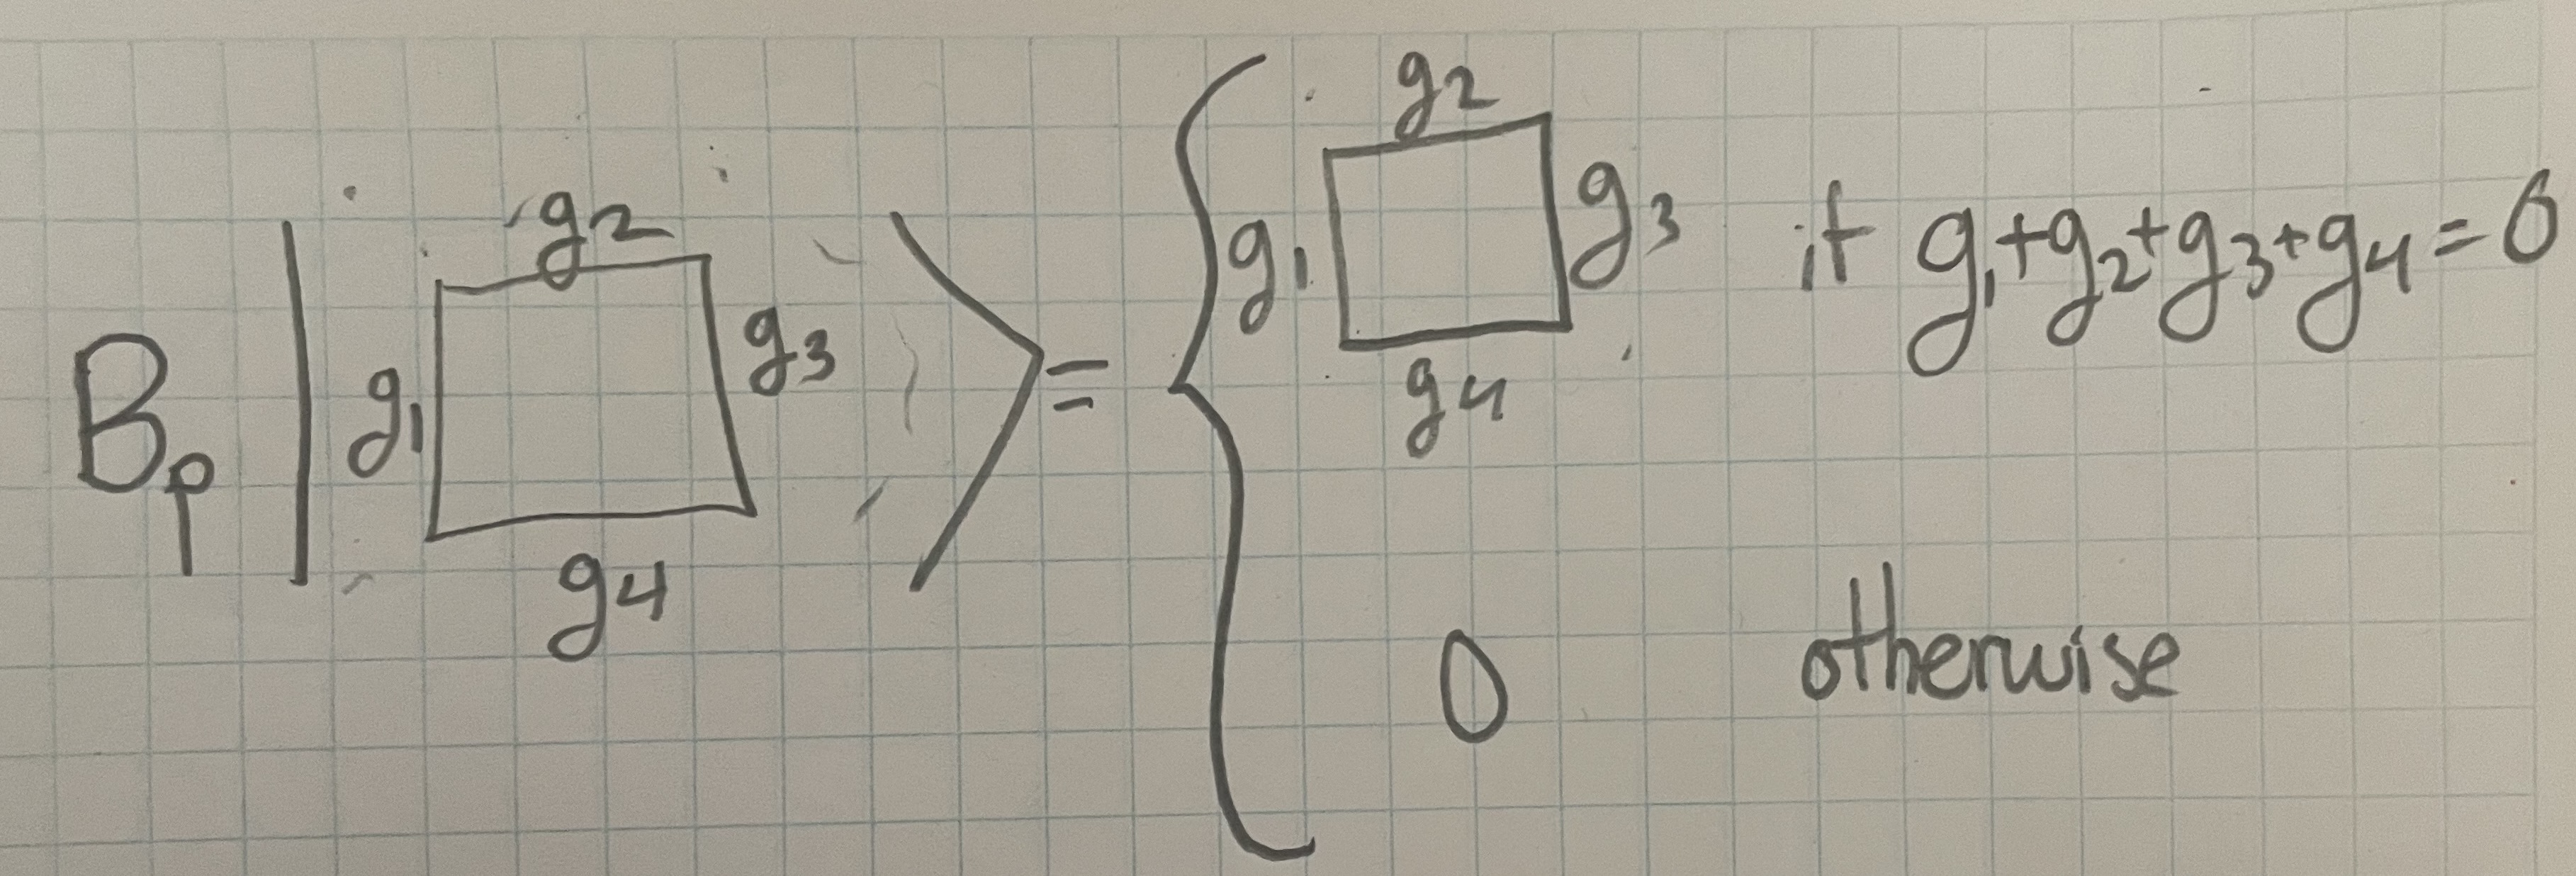
\includegraphics[scale=.04]{Bp-definition}
\end{center}
\end{figure}

In the present case, $B_p$ has a more workable expressing that is symmetric to our description of $B_p$. Define

\begin{align*}
\sigma_Z:\CC^2&\xrightarrow{}\CC^2.\\
\ket{0}&\mapsto \ket{0}\\
\ket{1}&\mapsto -\ket{1}
\end{align*}

Philosophically, it is useful to interpret $\sigma_Z$ as acting as $\ket{g}\mapsto \chi(g)\ket{g}$ where $\chi:\ZZ_2\to\CC^\times$ is the unique nontrivial character of $\ZZ_2$, $\chi(0)=1$, $\chi(1)=-1$. Since $\chi$ is a group isomorphism, for any $g_1,g_2,g_3,g_3\in G$ we have an equivalence

$$g_1+g_2+g_3+g_3=0 \iff \chi(g_1)\chi(g_2)\chi(g_3)\chi(g_4)=1.$$

Defining an auxillary $B_{p,1}$, we thus find the following expression for $B_p$:

\begin{align*}
B_{p,1}=\bigotimes_{\substack{\text{edges} \\ \text{bounding }p}}\sigma_Z, && B_p=\frac{1}{2}\left(I + B_{p,1}\right).
\end{align*}

For simplicity, we will often rewrite the Hamiltonian as

$$H=\frac{1}{2}\sum_{\text{vertices }v}(1-A_{v,1})+\frac{1}{2}\sum_{\text{plquettes }p}(1-B_{p,1}).$$

The matrices $\sigma_X$ and $\sigma_Z$ we defined are known as \textit{Pauli matrices}. They are extremely common across formulae in quantum mechanics - this is another reason that the toric code is so ammenable to error correction applications. The basic properties of these matrices are summarized below:

\begin{proposition}$\,$
\begin{enumerate}[(a)]
\item The operators $\sigma_X$ and $\sigma_Z$ are simultaneously unitary and Hermitian;
\item $\sigma_X^2=\sigma_Z^2=I$;
\item $\sigma_X \sigma_Z = - \sigma_Z \sigma_X$;
\end{enumerate}
\end{proposition}
\begin{proof}.[WORK: do proof]
\end{proof}

An important thing to note is that $A_{v,1}$ and $B_{p,1}$ commute, despite the fact that $\sigma_X$ and $\sigma_Z$ anticommute. The fact that they commute follows from Proposition [ref], though it fruitful to reavulate that proposition in this present context. The important fact is that given any vertex $v$ on the exterior of any face touching $p$,  there are an \textit{even number} of edges which both touch $v$ and bound $p$. Hence, the number of tensor factors in which $A_{v,1}$ and $B_{p,1}$ anticommute is even, and hence overall they commute.

The last step in reinterpreting our general theory of Kitaev quantum double models to the toric code is computing the ground space. We observe that since $\ZZ_2$ is abelian acting by conjugation does nothing, and hence

$$\Hom(\pi_1(T^2,v), \ZZ_2)/\left(\substack{\text{simultaneous} \\ \text{conjugation}}\right)=\Hom(\pi_1(T^2,v), \ZZ_2).$$

Seeing as we are no longer modding out by conjucation, the group operation on $\ZZ_2$ extends to a group operation on $\Hom(\pi_1(T^2,v), \ZZ_2)$. Hence this space forms an abelian group, which we denote

$$H^1(T^2,\ZZ_2)=\Hom(\pi_1(T^2,v), \ZZ_2)=(\text{flat $\ZZ_2$-colorings})/(\text{gauge transformations}).$$

[WORK: maybe set notation and write out four elements explicitely? Might be too much.]

This is the \textit{cohomology group of $T^2$ with coeffecients in $\ZZ_2$}. Since $\pi_1(T^2,v)\cong \ZZ^2$, we conclude that

$$H^1(T^2,\ZZ_2)\cong \ZZ_2^2.$$

Hence, we obtain the following:

\begin{proposition} The $0$-eigenspace of $H$ is four dimensional. It is spanned by the vectors

$$\ket{C}=\frac{1}{\sqrt{|C|}}\sum_{\gamma\in C}\ket{\gamma}$$

for $C\in H^1(T^2,\ZZ_2)$.
\end{proposition}
\begin{proof}.[WORK: do proof]
\end{proof}

\subsubsection{Anyons in the toric code}

We now turn to analysing anyons in the toric code - localized excitations which behave as quasiparticles. Keeping in line with general principles about the Kitaev quantum double model, given a state $\ket{\psi}\in \NN$ we say that there is an anyon at vertex $v$ if $A_v\ket{\phi}=0$, and we say that vertex $v$ is unnoccupied if $A_v\ket{\phi}=\ket{\psi}$. Similarly, we say that there is a quasiparticle at plaquette $p$ if $B_p\ket{\psi}=0$ and that plaquette $p$ is unoccupied if $B_p\ket{\psi}=\ket{\psi}$. In summary,

\begin{align*}
\text{$\ket{\psi}$ has anyon at $v$}\iff A_v\ket{\psi}&=0 \iff A_{v,1}\ket{\psi}=-\ket{\psi}\\
\text{$\ket{\psi}$ has anyon at $p$}\iff B_p\ket{\psi}&=0 \iff B_{p,1}\ket{\psi}=-\ket{\psi}.
\end{align*}

We call the anyons at vertices \textit{vertex type} or \textit{$Z$-type} anyons, and we call the anyons at faces \textit{plaquette type} or \textit{$X$-type} anyons. Our key observation is that applying $\sigma_X$ and $\sigma_Z$ gives total control over the behavior of anyons. Namely, applying $\sigma_X$ or $\sigma_Z$ in the correct circumstates corresponds to creating, moving, and fusing anyons. This comes from the following computation. Given an edge $e$ in the lattice and an operator $U:\CC^2\to \CC^2$, denote by $(U)_e:\NN\to\NN$ the operator which applies $U$ on the tnesor factor of $\CC^2$ at edge $e$. We compute the following:

\begin{lemma} For any vertex $v$, edge $e$, plaquette $p$, we have

\begin{align*}
A_v  (\sigma_X)_e=(\sigma_X)e A_v, && B_p (\sigma_Z)_e=(\sigma_Z)e B_p,
\end{align*}

\begin{equation*}
A_v (\sigma_Z)_e=
\begin{cases}
- (\sigma_Z)_e A_v & \text{if $e$ touches $v$}\\
(\sigma_Z)_e A_V & \text{otherwise}
\end{cases}
\end{equation*}

and

\begin{equation*}
B_p (\sigma_X)_e=
\begin{cases}
- (\sigma_X)_e B_p & \text{if $e$ bounds $p$}\\
(\sigma_X)_e B_p & \text{otherwise}
\end{cases}
\end{equation*}


\end{lemma}
\begin{proof}.[WORK: do proof]
\end{proof}

Suppose that $\ket{\psi}$ is a state with no anyons -that is, a ground state. Given any edge $e$, the state $(\sigma_X)_e \ket{\psi}$ will not be a ground state. In particular, it will no longer commute with $B_p$ at the two plaquettes touching $e$. In this way, applying $\sigma_X$ to the edge $e$ spontanously created a pair of $X$-type anyons around it. Similarly, the staet $(\sigma_Z)_e\ket{\psi}$ will no longer commute with the $A_v$ operators at the two vertices touching $e$. Hence applying $\sigma_Z$ to the edge $e$ spontaneously created a pair of $Z$-type anyons around it. Applying further $\sigma_Z$ and $\sigma_X$ operators has the effect of chaning the quasiparticle content of the state further. If both the adjacent sites are unnoccupied then applying the operator will create a pair of anyons, if one of the sites is occupied then applying the operator will move the anyon from the occupied site to the unoccupied site, and if both of the sites are occupied then applying the operator will annhilate the anyons. We demonstrate this in some examples below

\begin{figure}[h]
\begin{center}
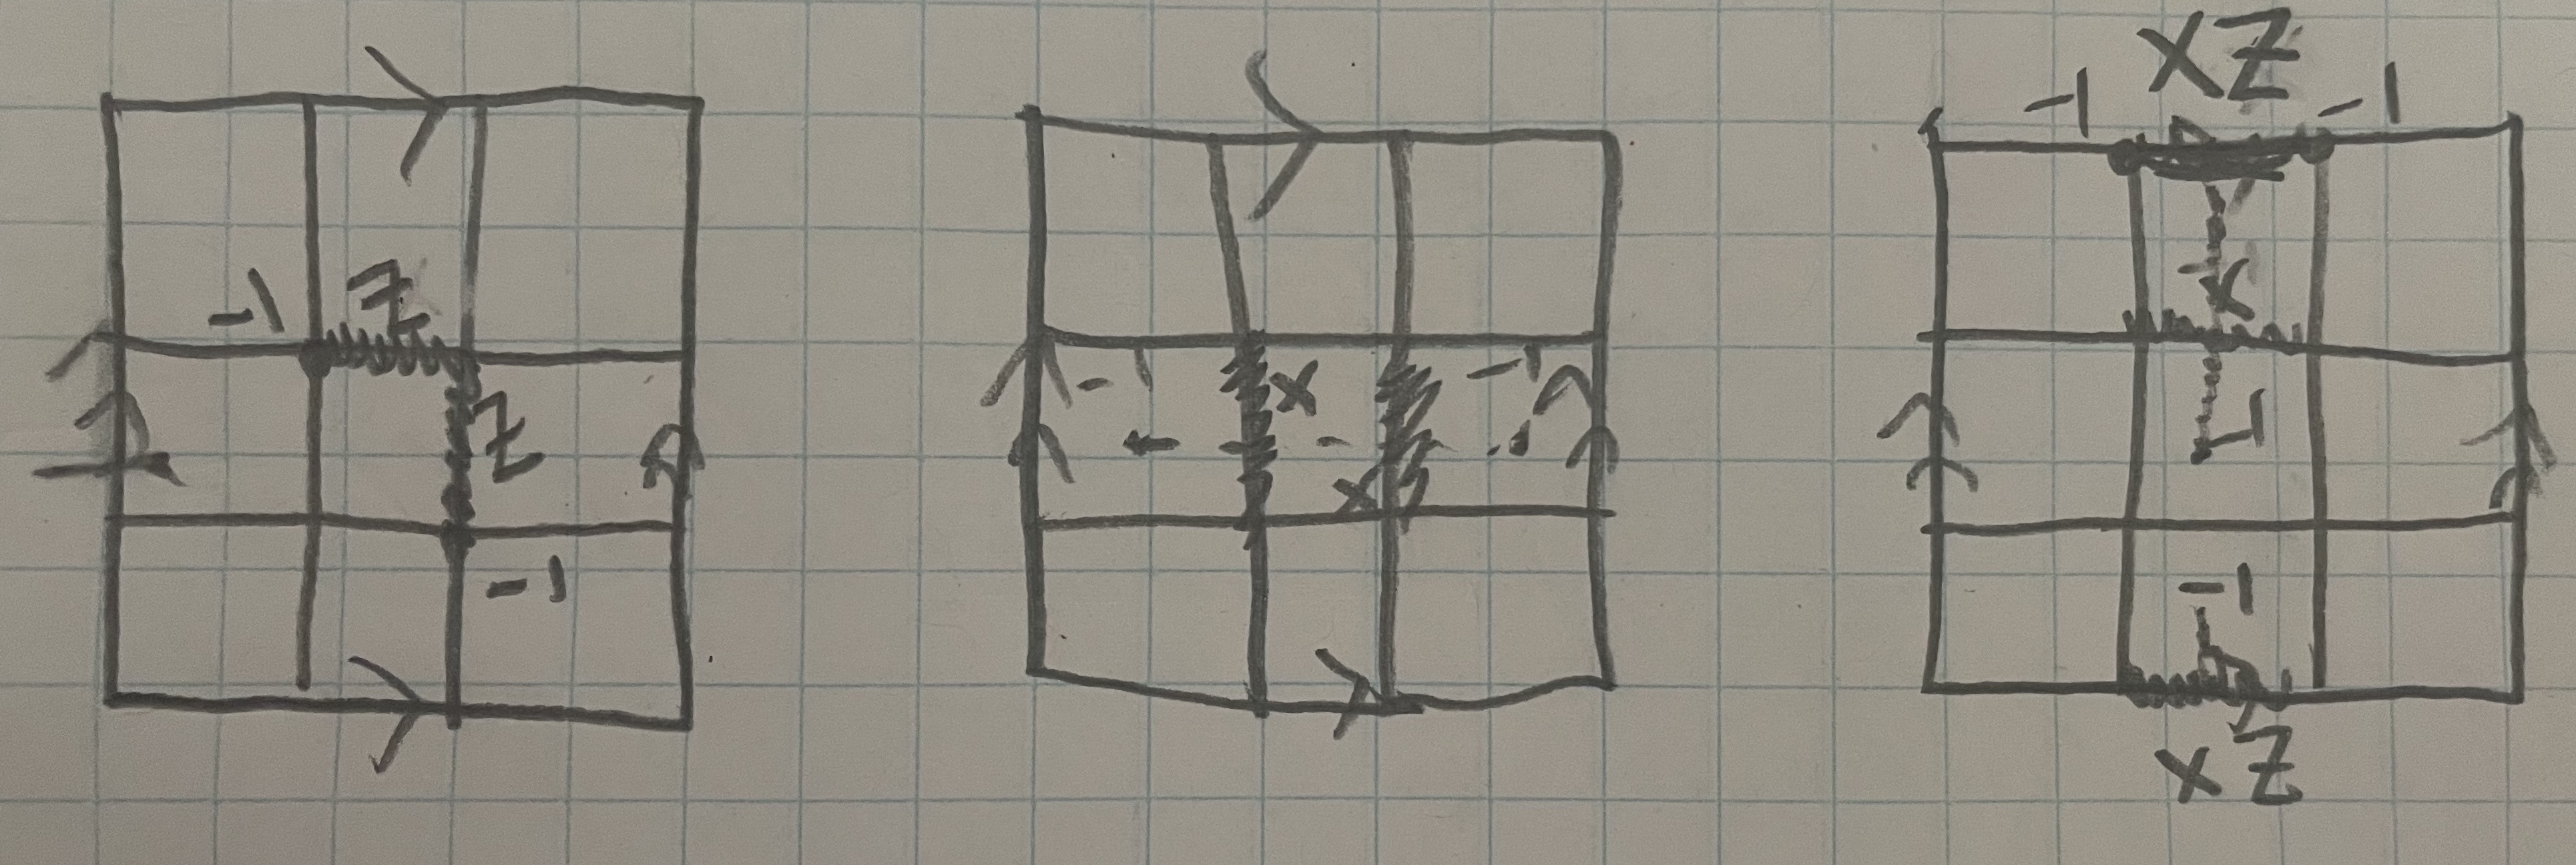
\includegraphics[scale=.04]{anyon-examples}
\end{center}
\end{figure}

We can use this idea of anyons to fully solve the toric code. We introduce some terminology and notation. Given an energy eigenstate $\ket{\psi}$, there is an associated map $\lambda: (\text{vertices})\sqcup (\text{plaquettes})\to \{\pm 1\}$ defined by the relation $A_{v,1}\ket{\psi}=\lambda(v)\ket{\psi}$, $B_{p,1}\ket{\psi}=\lambda(p)\ket{\psi}$. We call maps $\lambda: (\text{vertices})\sqcup (\text{plaquettes})\to \{\pm 1\}$ \textit{syndromes}, and the map associated to $\ket{\psi}$ is the \textit{syndrome of $\ket{\psi}$}. These syndromes allow us to speak intelligently about the locations of anyons within a state. For any syndrome $\lambda$, define

$$\NN_\lambda=\left\{\ket{\psi}\left| \text{syndrome of $\ket{\psi}$ is $\lambda$}\right.\right\}.$$

It is clear that

$$\NN=\bigoplus_{\text{syndromes $\lambda$}}\NN_\lambda$$

and

$$\C=\NN_{\sigma(v)=\sigma(p)=1 \,\, \forall v,p}$$

The following proposition and its proof give a complete description of the eigenstates and eigenvalues

\begin{proposition}The dimension of $\NN_{\lambda}$ is $4$ if the number of vertices $v$ and plaquettes $p$ for which $\lambda(v)=-1$ and $\lambda(p)=-1$ are both even, and the dimension of $\NN_{\lambda}$ is zero otherwise. The eigenvalue of every vector in $\NN_{\lambda}$ is equal to the total number of anyons in the system.
\end{proposition}
\begin{proof}.[WORK: do proof]
\end{proof}

The anyons in the toric code are interesting objects in their own right. For example, we can analyse what happens when we braid anyons. Suppose that $\ket{\psi}$ is a state with one $X$-type anyon and one $Z$-type anyon at adjacent sites. That is, the $X$-type anyon is at a vertex $v$ touching a plaquette $p$. Moving the $Z$-type anyon around the $X$-type anyon corresponds to applying $\sigma_Z$ to the edges around the $X$-type anyone one by one. In other words, the operator required to move the $Z$-type anyon is the tensor product of $\sigma_Z$ along the edges bounding $p$. However, by definition, this operator is exactly $B_{p,1}$. We know that $B_{p,1}\ket{\psi}=-\ket{\psi}$ by the definition of having an anyon at plaquette $p$. Hence, we conclude that \textit{moving a $Z$-type anyon around an $X$-type anyon results in a phase of $-1$}. Similarly, we oberve that moving a $Z$-type anyon around an $X$-type anyon also results in a phase of $-1$, as shown below:

\begin{figure}[h]
\begin{center}
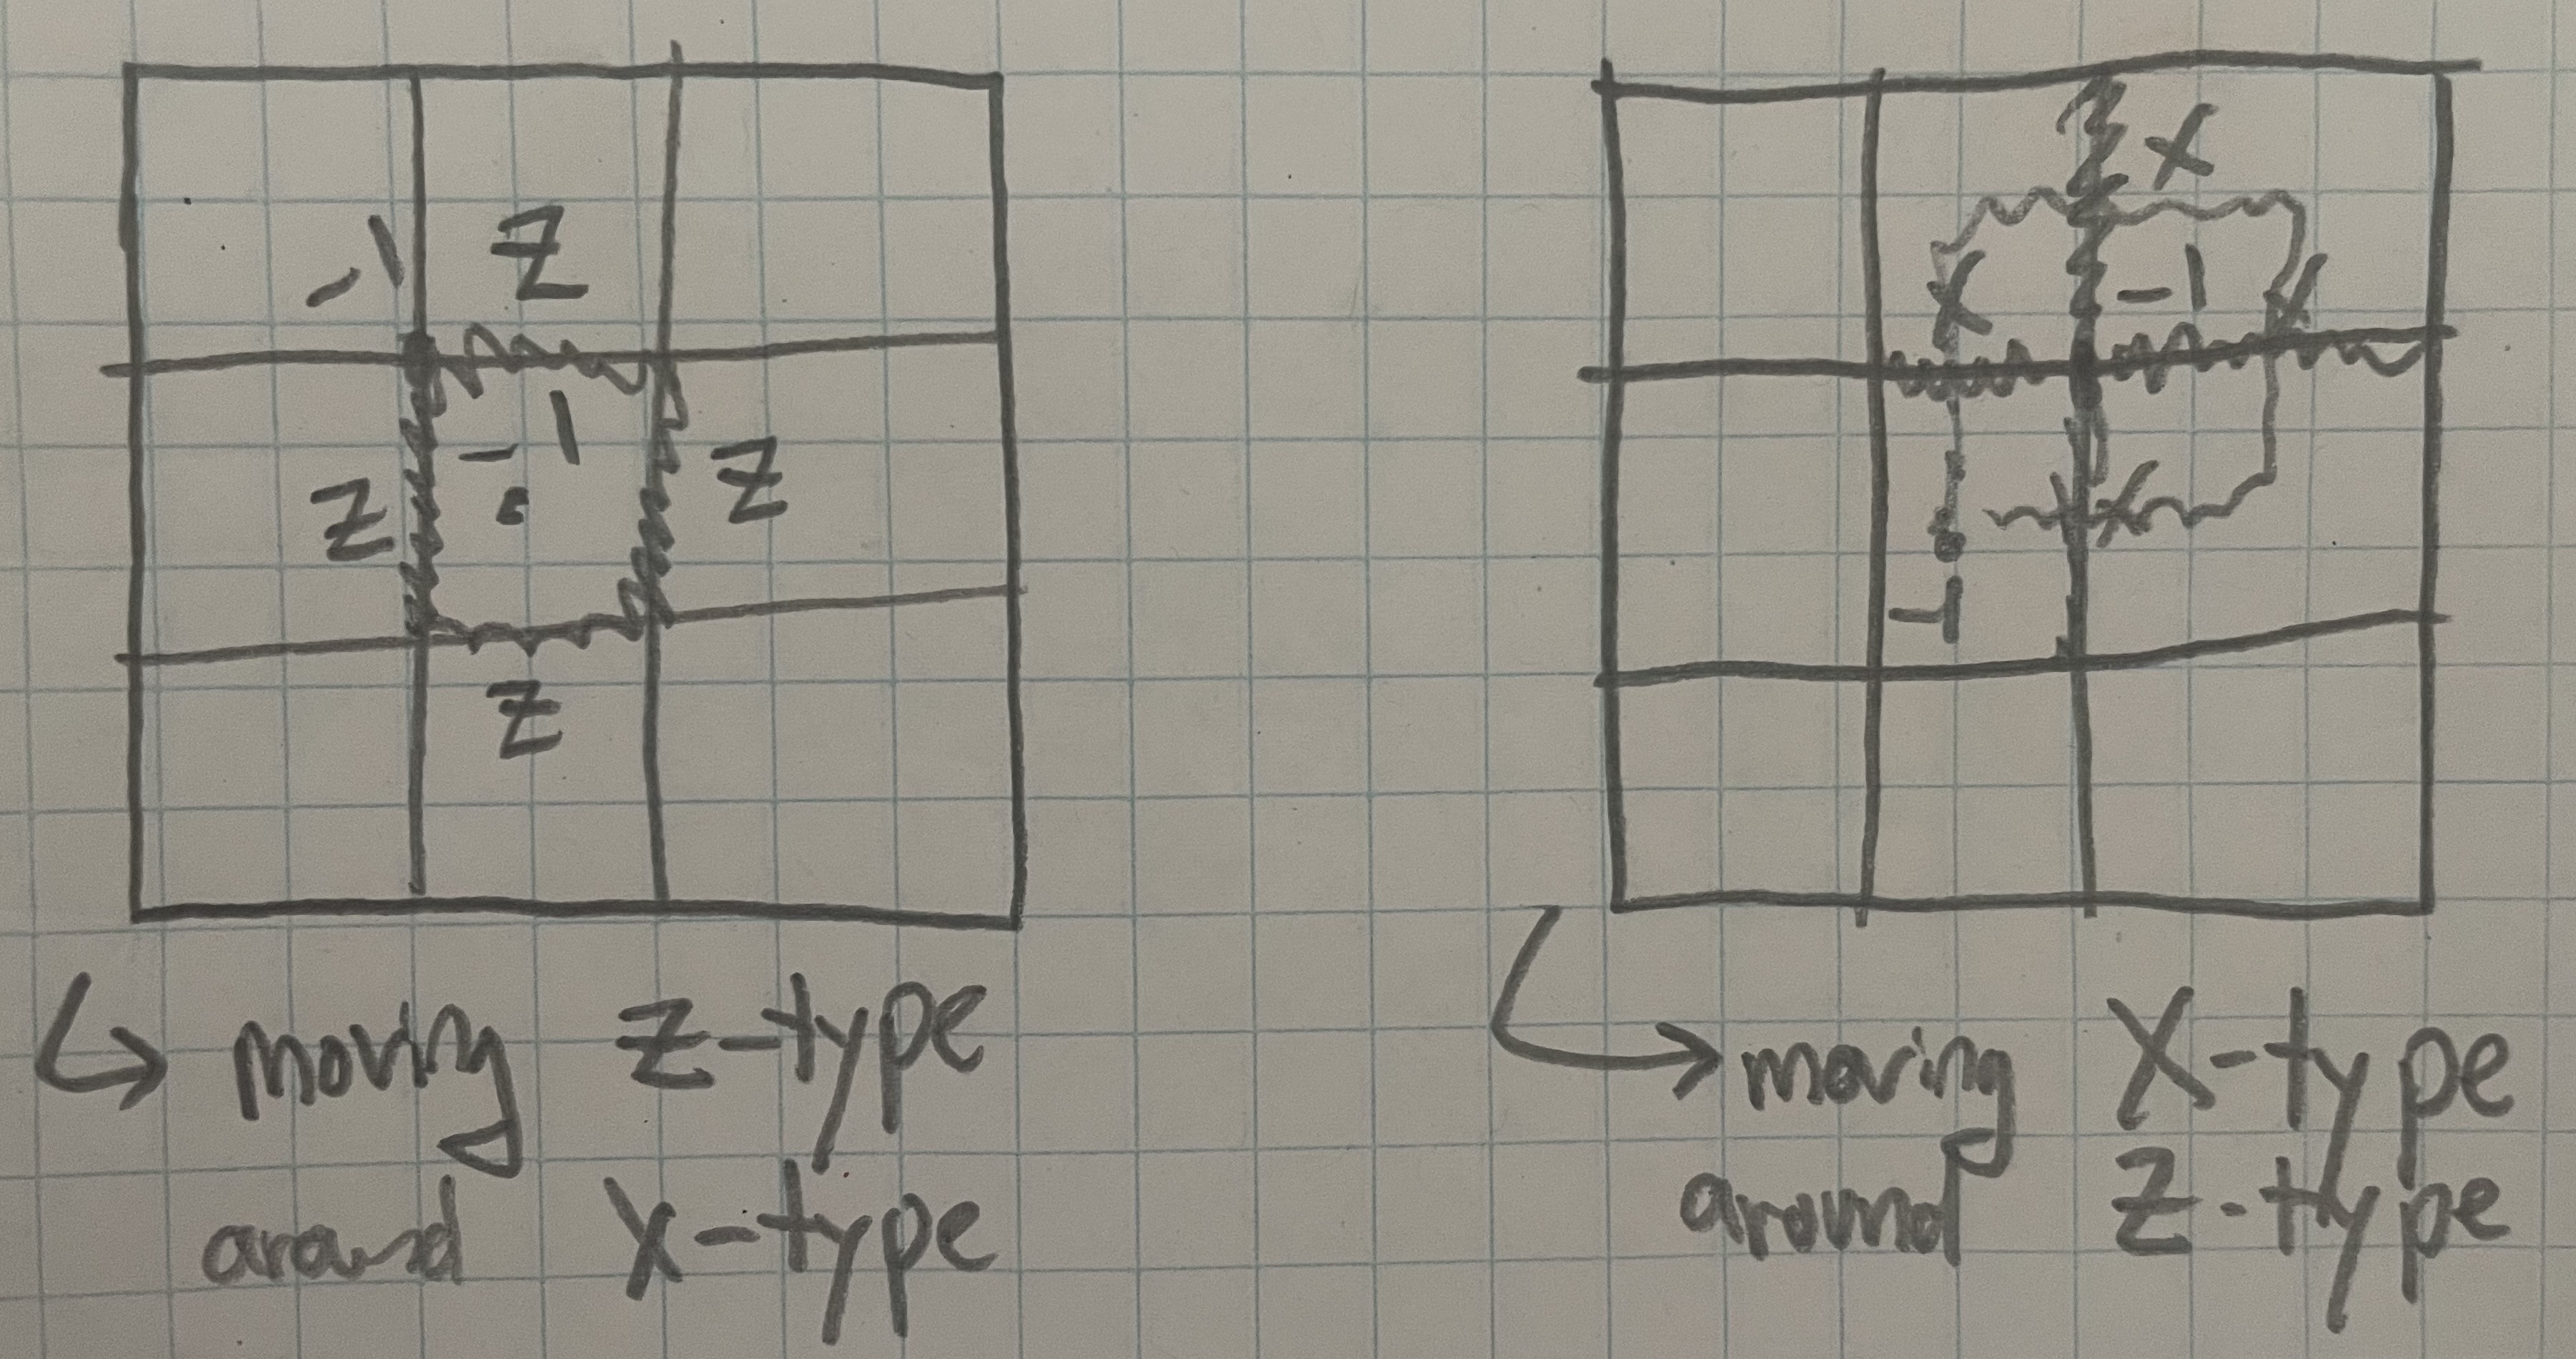
\includegraphics[scale=.04]{mutual-anyon-stats}
\end{center}
\end{figure}

We codify this in a proposition. However, seeing as we have not defined what it means for one anyon to move ``around" another, we can only state it on the physical level of rigor:

\begin{propositionph} Moving $X$-type anyons around $Z$-type anyons results in a phase of $-1$. Similarly, moving $Z$-type anyons around $X$-type anyons results in a phase of $-1$.
\end{propositionph}
\begin{proof}.[WORK: do proof]
\end{proof}

There is also an interesting action of anyons on the ground states of the toric code. This action is performed by starting with a ground state, creating anyon pairs, and then moving one of the anyons in that pair around a non-trivial loop around the torus, and then annhilating it back with its partner. This process is shown below:

[WORK: include diagram]

We can describe this action completely as fllows:

[WORK: give the picture of TQC by moving anyons around in proposition-format]

This concludes our picture of anyons in the toric code.

\subsection{Non-abelian anyons}

\subsubsection{Principles of anyons}

We recall that \textit{anyons} are localized excitations in topologically ordered systems. They behave as quasiparticles. In the previous section we analysed the toric code, and explored the behavior of anyons in the toric code. There were two types of anyons : $X$-type and $Z$-type. Each anyon type was its own antiparticle. The anyons braided trivially with themselves, but bothing any type of anyon around the other results in a $-1$ phase. In this subsection we will discuss the general theory of anyons which the toric code is part of.

To begin, we will recall some broader themes in particle physics. The modern world of particle physics is dominated by the \textit{standard model}. This model is a quantum field theory which describes the fundamental particles of the universe and how they interact. There are 61 different elementary particle types, each taking part in a broad explanation of the fundamental forces of the unvierse. An important feature of the standard model is a dichotemy between \textit{bosons} and \textit{fermions}. When bosons are exchanged it does not affect their underlying wave function, and when fermions are exchanged it results in a phase of $-1$.

Put more concretely, consider some particle type $A$. Let $V_2$ denote the Hilbert space of a system containing $2$ identical $A$-type particles. We can consider a unitary operator $\swap:V_2\to V_2$, which encodes the action on $V_2$ induces by taking the two particles and swapping their positions. It is a feature of the standard model that the details of how this swap doesn't change the action on $V_2$ - there is a well-defined $\swap$ map which only depends on the topology of the swap. It is a fact from the standard model that either $\swap$ is the identity map or $\swap$ is the unitary which multiples phases by $-1$. If $\swap=I$ then we call $A$ a boson, and if $\swap=-I$ we call $A$ a fermion.

We now explain why all of the particles in the standard model are bosons or fermions. The general idea is as follos. If we swap twice, then the particles go back to their original position. Hence, $\swap^2=I$. Hence, $\swap=I$ or $\swap=-1$. This general arguments works well for the standard model, but it has several subtleties which are important to highlight. Firstly, just because $\swap^2$ brings the particles got back where they started doesn't mean that the path they took has trivial topology. In space time it looks like the following:

\begin{figure}[h]
\begin{center}
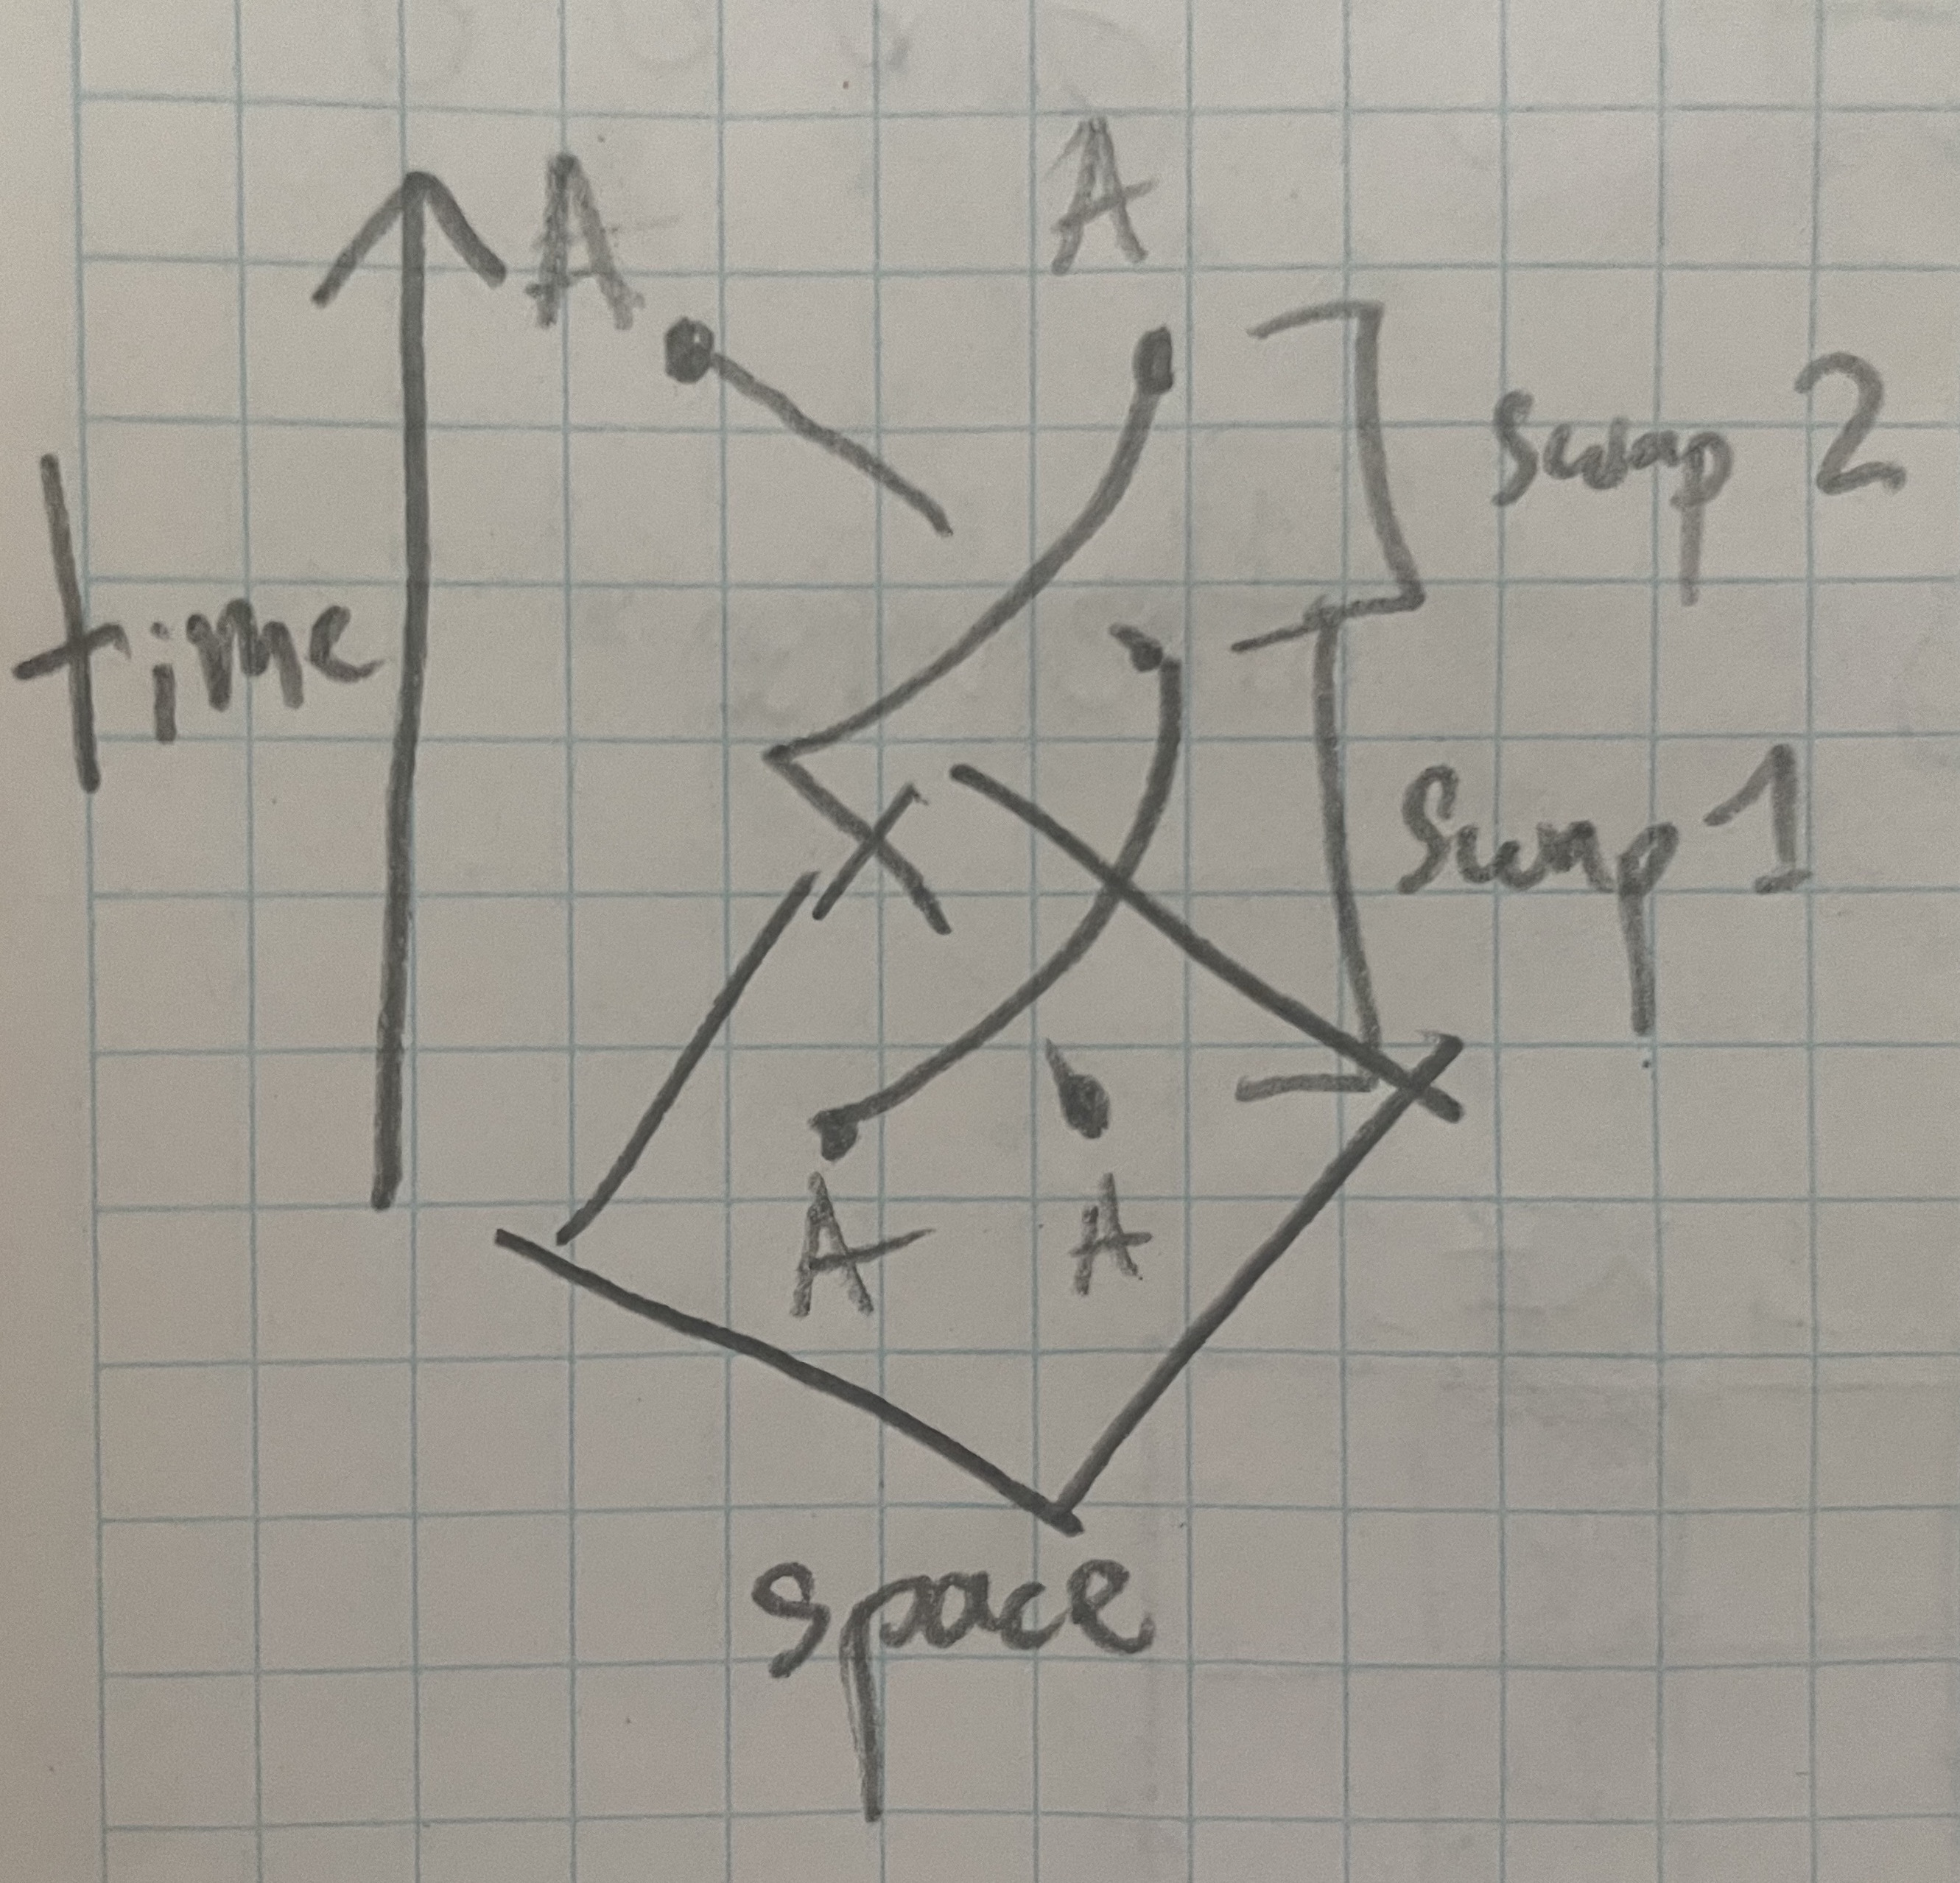
\includegraphics[scale=.04]{two-swaps}
\end{center}
\end{figure}

If physical space had two dimensions, then this is a topologically nontrivial braid. The important feature of the standard model is that it has three space dimensions. In three space dimensions, the double swap has trivial topology: the two strands can be moved smoothly past each other without intersected by pushing them into different parts of the third dimension. In general, the possible ways that $n$ particles can move around each other in two dimensions is the braid group $B_n$ we defined in section [ref], whereas the ways that particles can move around each other in three dimensions degenerates to the symmetric group $S_n$. Let $V_n$ denote the $n$ particle system of $n$ identical particles of type $A$. In two dimensions, moving the $n$ particles around in braids gives a representation

$$B_n\xrightarrow{}U(V_n)$$

whereas in three dimensions it gives a representation

$$S_n\xrightarrow{}U(V_n).$$

This difference between $B_n$ and $S_n$ causes a huge change between what is possible in three dimensions versus two dimensions. For instance, suppose that our braids only act by phases. That is, the image of the particle statistics maps lie in $U(1)\hookrightarrow{}U(V_n)$. In $B_n$, there is such a representation corresponding to any phase $\omega\in U(1)$. In this representation, exchanging two identical particles results in a phase $\omega$. In $S_n$, there are only two such representations: the trivial representation and the sign representation, corresponding to the phases $+1$ and $-1$ accordingly. These two representations correspond to bosons and fermions.

The last part of the explanation of why all particles in the standard model are fermions and bosons is more subtle. From our above discussion, it is clearly a-priori possible that there could be particles in 3 spacial dimensions which act by non-trivial higher dimensional representations of $S_n$. It turns out that this doesn't happen, and in fact it \textit{can't} happen in any (3+1)D quantum field theory, but this is for much more subtle reasons [WORK: add refs]. This doesn't mean that there aren't any models in 3 dimensions with quasiparticles that aren't bosons or fermions - these certainly exist [WORK: add refs]. It just means that these models are more rare and require some amount of trickery. The fact that all fundamental particles in (3+1)D quantum field theories are fermions or bosons is one of the main reasons we are working with (2+1)D systems in this book.

The toric code already demonstrates how particles can behave in ways in (2+1)D which are impossible in (3+1)D. When an $X$-type particle is moved all the way around a $Z$-type particle it results in a phase of $-1$. Of course, in (3+1)D moving one particle all the way around another is topologically trivial and hence would have to result in a phase of $+1$.

It is from this discussion that the name \textit{anyon} arrises. Bosons have $+1$ exchange phases, fermions have $-1$ exchange phases. Anyons, excitations in topolgoically ordered systems, can have \textit{any} exchange phase. Hence, \textit{any}on. Additionally, there are many natural systems which exhibit anyons whose exchange statistics results in higher dimensional representations of the braid group. These are known as \textit{non-abelian} anyons. Anyons which act by phases are known as \textit{abelian} anyons.

One intuition for the name abelian versus non-abelian comes from the Kitaev quantum double model. We will see that the Kitaev quantum double model based on a finite group $G$ hosts non-abelian anyons if and only if $G$ is non-abelian. Alternatively, you could motivate the name by noticing that an anyon is abelian if and only if the image of its associated braid group representation is abelian.

The algebraic theory of anyons is the heart and soul of topological order. This is quantified by the fact that our algebraic description of topological order will really be an algebraic description of anyons, and we will be asserting implicitely that describing the behavior of the anyons is enough to describe the topological order.

\subsubsection{The algebraic structure of discrete gauge theory}

.[WORK: go from KQDM to $G$-crossed $G$-representations. Doing this in the most painless way is subtle, and will probably require two subsections. By the end we should have the category $\D(G)$ as a set, with morphisms motivated.]

$\newline$
\fbox{\parbox{\dimexpr\linewidth-2\fboxsep-2\fboxrule\relax}{

\begin{center}
\textbf{History and further reading:}\\
\end{center}

The term topological order was first used in 1972 by Kosterlitz and Thouless to describe topological classical systems of the sort discussed in Chapter [ref] \cite{kosterlitz2018ordering} . The term has since evolved, and was re-coined in 1989 by Xiao-Gang Wen to describe the sort of topological classical systems defined in this chapter \cite{wen1989vacuum}.

$\newline$
The history anyons is distinct from the history of topological order. It was first noted in 1976  in a paper of Leinass and Myrheim that the classification of particles in terms of fermions and bosons broke down in two dimensions \cite{leinaas1977theory}. The subject of anyons was then taken over by Wilczek who published a series of seminal papers on the topic \cite{wilczek1982magnetic, wilczek1982quantum, arovas1984fractional}. It was in these papers that Wilczek observed that anyons were present in the quantum Hall effect, and hence connected the theory of anyons and topological order together.

[WORK: what is the history of gauge theory, and when was it introduced to the picture? A great reference is the de Wild Propitius and Bais survey. Also should mention Kitaev's paper again.]

}}


$\newline\newline$

\large \textbf{Exercises}:\normalsize

\begin{enumerate}[\thesection .1.]

\item For vertices $v$ and plaquettes $p$, define

\begin{align*}
A'_{v,1}=\bigotimes_{\substack{\text{edges} \\ \text{touching }v}}\sigma_Z, && A'_v=\frac{1}{2}\left(I + A'_{v,1}\right),
\end{align*}

\begin{align*}
B'_{p,1}=\bigotimes_{\substack{\text{edges} \\ \text{bounding }p}}\sigma_X, && B'_p=\frac{1}{2}\left(I + B'_{p,1}\right),
\end{align*}

and

$$H'=\sum_{\text{vertices }v}(1-A'_v)+\sum_{\text{plaquettes }p}(1-B'_p).$$

Define $M:\CC^2\to \CC^2$ by $M(\ket{0})=\frac{1}{\sqrt{2}}(\ket{0}+\ket{1})$ and $M(\ket{1})=\frac{1}{\sqrt{2}}(\ket{0}-\ket{1})$. Show that

$$\sigma_X=M\sigma_ZM^{-1},\,\, \sigma_{Z}=M\sigma_X M^{-1},$$

and show that $H$ and $H'$ are similar in the sense that $H'=MHM^{-1}$. Use this to conclude that all basis independent properties of the toric code are formally symmetric by replacing $\sigma_X$ with $\sigma_Z$. For example, conclude that the codespace of $H'$ is 4 dimensional.

\end{enumerate}